\documentclass[intlimits, 9pt, unicode]{beamer} 

\mode<presentation>
\usepackage[T2A]{fontenc}
%\usepackage[cp1251]{inputenc}
\usepackage[utf8]{inputenc}
\usepackage[russian]{babel}
\usepackage{graphicx}
\usepackage{amssymb}
\usepackage{amsthm}

\usefonttheme[onlymath]{serif}

\usepackage{beamerthemesplit}

\usetheme{Warsaw}
\setbeamertemplate{page number in head/foot}[totalframenumber]

\setbeamercovered{transparent}
\beamertemplatenavigationsymbolsempty



\title{Deciphering internet traffic patterns}
\author{Nina Golyandina, Kliment Merzlyakov}
\institute{Saint Petersburg State University \\
     Statistical modeling department \\
    Airpush
}
\date{
    Unlock customer lifetime value with advanced statistical techniques\\
    London\\
    17.10.2018
}

\AtBeginSection[]{
  \begin{frame}
  \vfill
  \centering
  \begin{beamercolorbox}[sep=8pt,center,shadow=true,rounded=true]{title}
    \usebeamerfont{title}\insertsectionhead\par%
  \end{beamercolorbox}
  \vfill
  \end{frame}
}


\begin{document}

\begin{frame}
    \titlepage
\end{frame}

\begin{frame}
    \frametitle{Content}

    \begin{itemize}
    	\item Change point detection. General notes
	\item Mobile advertising data
        \item Change point detection techniques
        \item Applications to real data
    \end{itemize}
    
    
\end{frame}



\section{Change point detection. General notes}

% \begin{frame}
%     \frametitle{Example}
% 
%         \begin{figure}
%         \centering 
% 	\textbf{Volume of ads served for specific country}
%         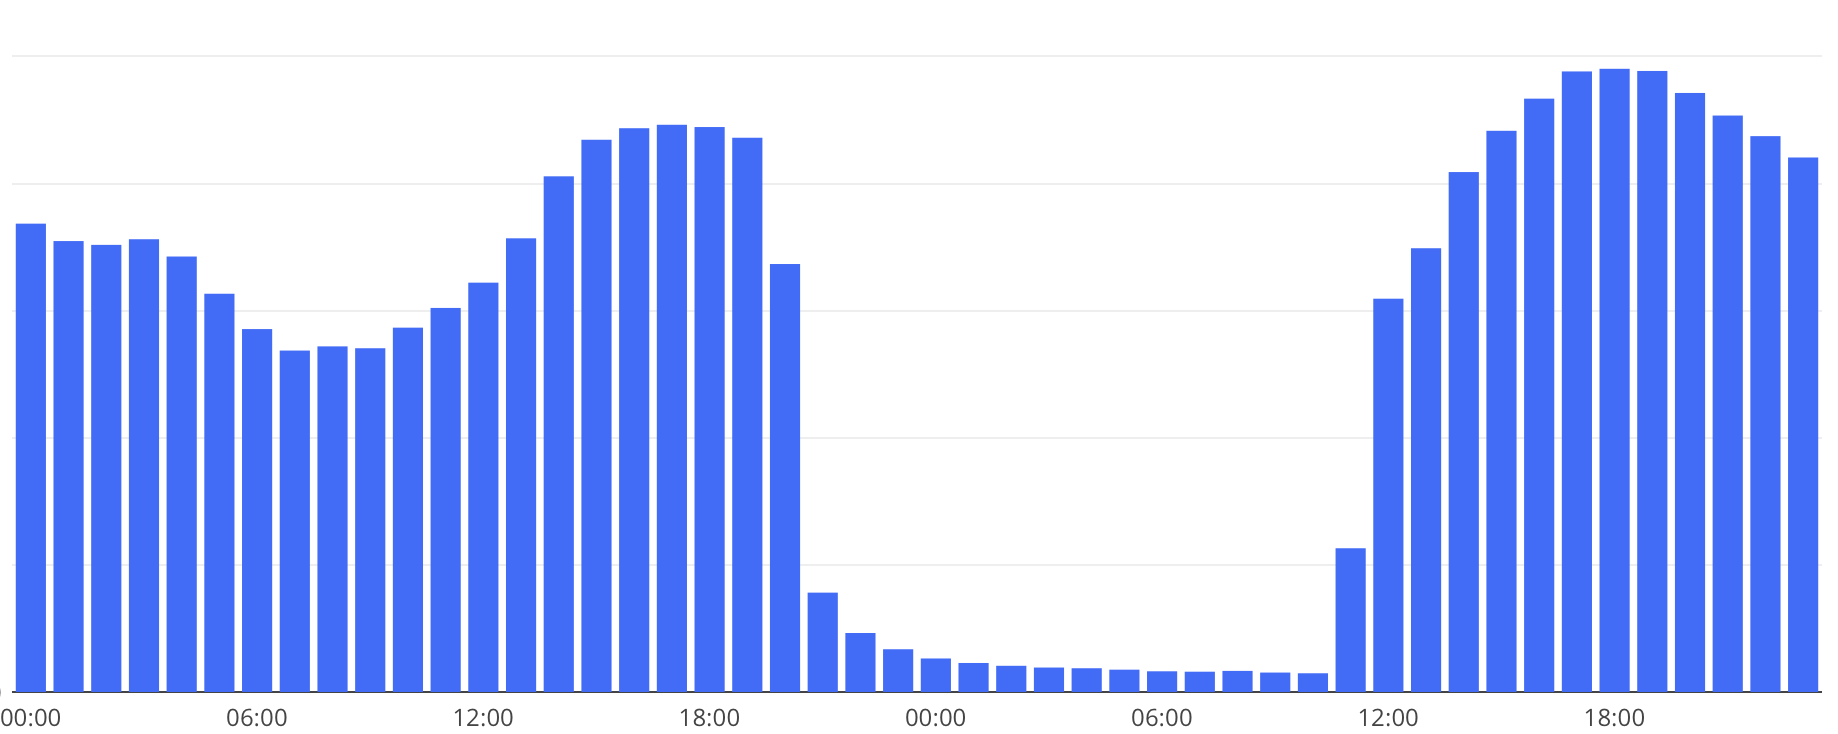
\includegraphics[height=4.5cm]{images/introduction_example}
% 	\end{figure}
	
%     \begin{itemize}
%     	\item Evening change of advertising software
% 	\item Fixed only at morning
% 	\item It's important to detect it automatically and correct it
%     \end{itemize}
% \end{frame}


\begin{frame}
    \frametitle{Changes in data}
    
       {\begin{columns}
        \begin{column}{5cm}
        User side changes
         \begin{itemize}
    		\item Application popularity
		\item Competition
		\item Applications' marketing activity
		\item ...
   	 \end{itemize}
        \end{column}

        \begin{column}{5cm}
        Advertising network side changes
         \begin{itemize}
    		\item New features released
		\item New advertisers onboarded
		\item New targeting strategy
		\item ...
   	 \end{itemize}
	 \end{column}
    \end{columns}}

 \end{frame}


\begin{frame}
    \frametitle{Time series}
	
    {\begin{columns}
        \begin{column}{5cm}
 Time series - is a sequence of numbers sorted by time (minute, hour, day, week, etc.)

\begin{table}[h!]
\centering
 \begin{tabular}{||c c||} 
 \hline
 Time & Data \\ [0.5ex] 
 \hline\hline
 17-Oct-2018 19:00 & 435 098 \\ 
 \hline
 17-Oct-2018 20:00 & 431 248  \\
 \hline
 17-Oct-2018 21:00 & 420 329  \\
 \hline
 ... & ... \\ [1ex] 
 \hline
\end{tabular}
\end{table}

	
 $ X = (x_1, x_2, ... , x_{N-1} , x_N)  $

        \end{column}

        \begin{column}{5cm}
Commonly time series can be decomposed $X = T + S + E$
        \begin{figure}
        \centering 
	\textbf{Time series. Decomposition example}
        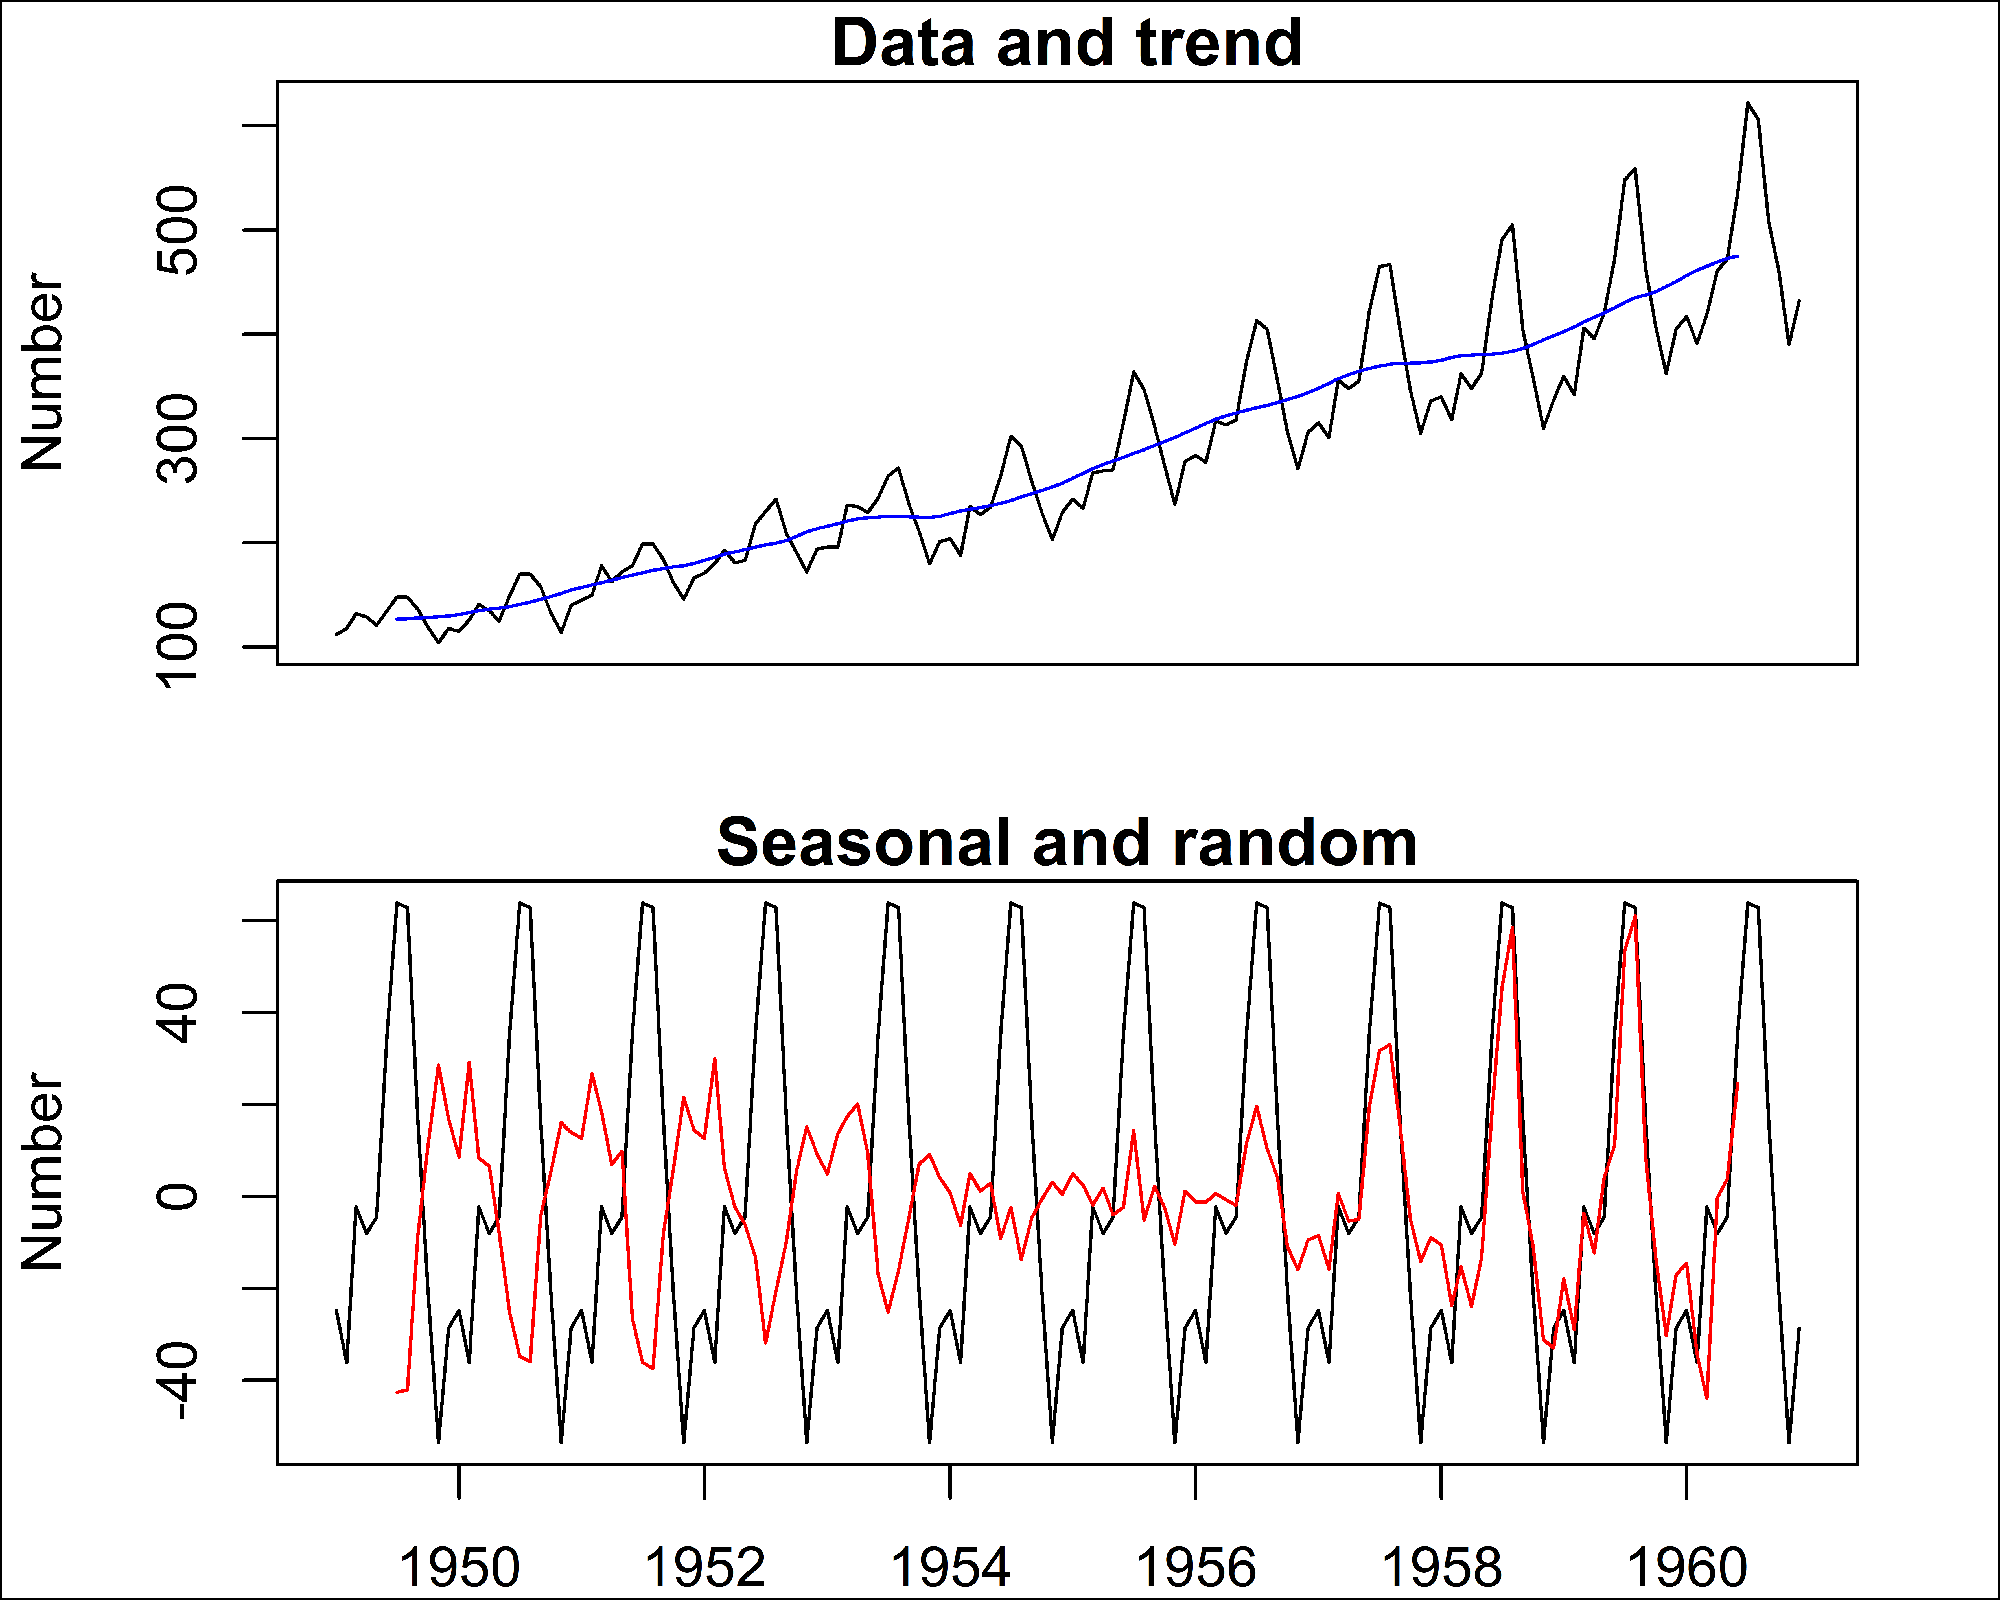
\includegraphics[height=4.5cm]{images/tsDecompPlot}
	\end{figure}
	
        \end{column}
    \end{columns}}
\end{frame}

\begin{frame}
    \frametitle{What is change point detection?}

    \begin{itemize}
    	\item Change point --- point in time series where some significant change in structure occurred
	\item Change point detection --- group of methods to find change points in time series
	\item Change points can be two types:
		\begin{itemize}
			\item Local --- anomaly or outlier
			\item Global --- change of time series structure 
		\end{itemize}
    \end{itemize}

    {\begin{columns}
        \begin{column}{5cm}
        \begin{figure}
        \centering 
	\textbf{Local change point}
        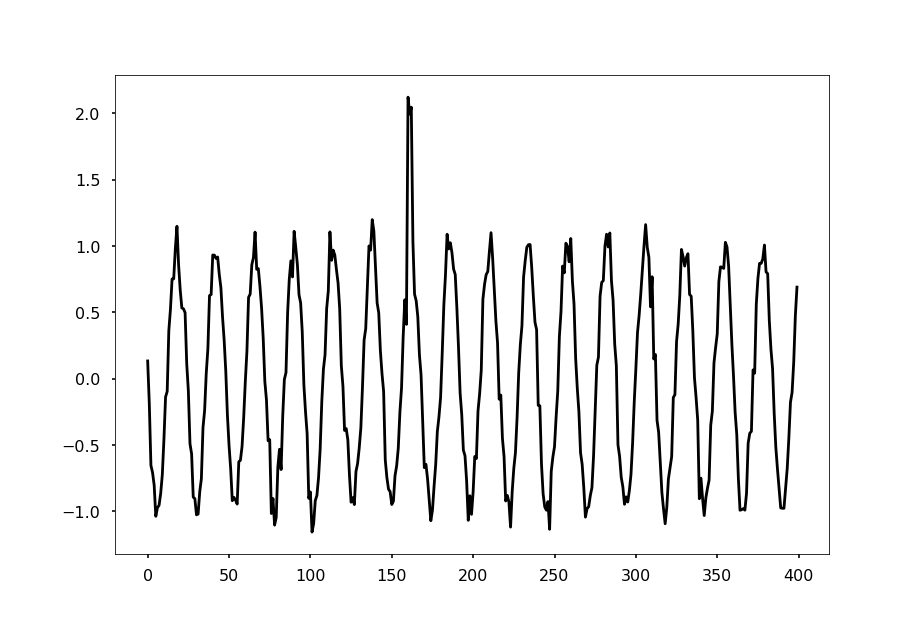
\includegraphics[height=3.5cm]{images/local_cp}
	\end{figure}
        \end{column}

        \begin{column}{5cm}
	\begin{figure}
    	\centering
	\textbf{Global change point}
        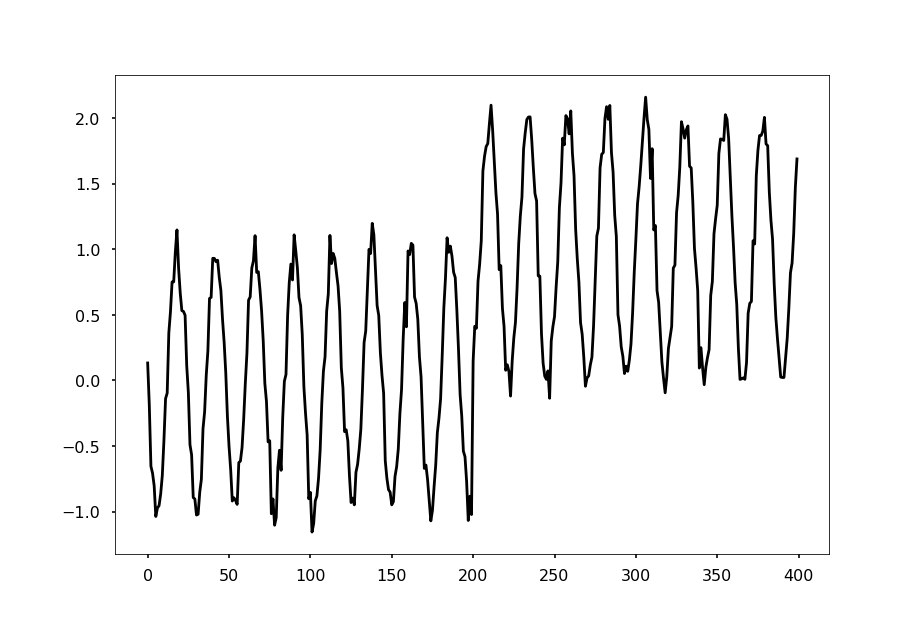
\includegraphics[height=3.5cm]{images/global_cp}
	\end{figure}
        \end{column}
    \end{columns}}
    
\end{frame}


\begin{frame}
    \frametitle{Motivation}
When it helps:
    \begin{itemize}
    	\item Forecasting
	\item Extracting trend more accurately
    	\item Searching issues in historical data 
	\item Reacting on changes quickly
    \end{itemize}
   
   
   \begin{columns}
        \begin{column}{5cm}
	\begin{figure}
		\textbf{Without CP detection}
		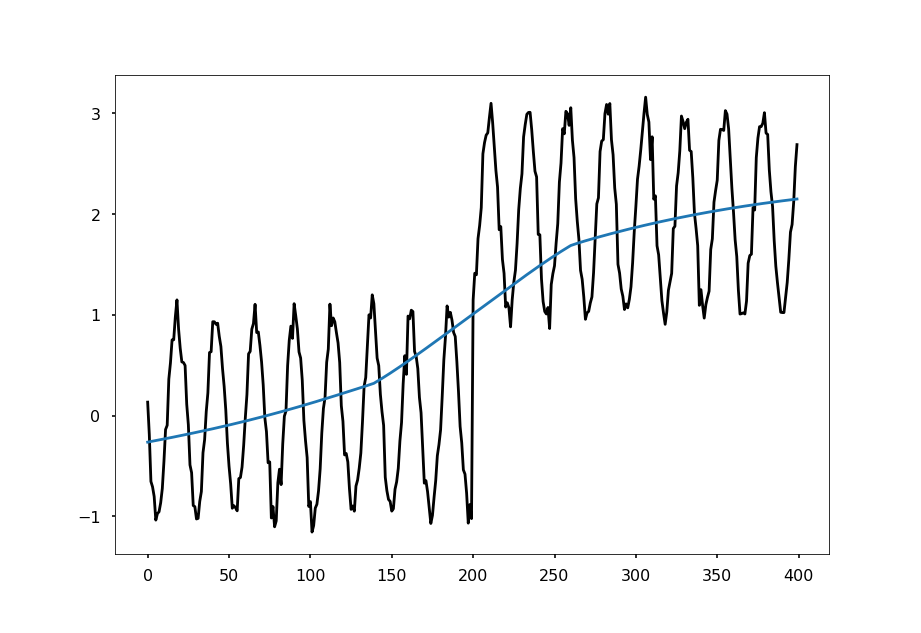
\includegraphics[height=3.5cm]{images/trend_fallacy}
	\end{figure}
        \end{column}
        
        \begin{column}{5cm}
	\begin{figure}
		\textbf{With CP detection}
		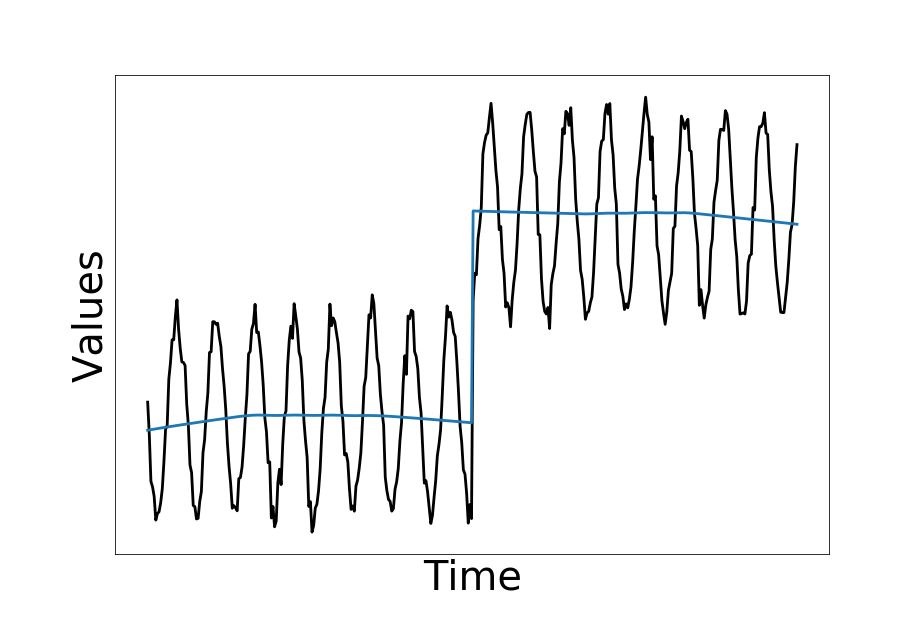
\includegraphics[height=3.5cm]{images/trend_succeed}
	\end{figure}
        \end{column}
    \end{columns}
    
What can we do:
    \begin{itemize}
    	\item Remove/change outliers or use robust methods
	\item Split time series and analyze separately
    \end{itemize}

\end{frame}


\begin{frame}
    \frametitle{Types of change points}

\begin{columns}
 \begin{column}{0.5\textwidth}
 
  \begin{columns}
      \begin{column}{0.3\textwidth}
      \centering
      Trend change
      \end{column}
      \begin{column}{0.5\textwidth}
      \begin{figure}
		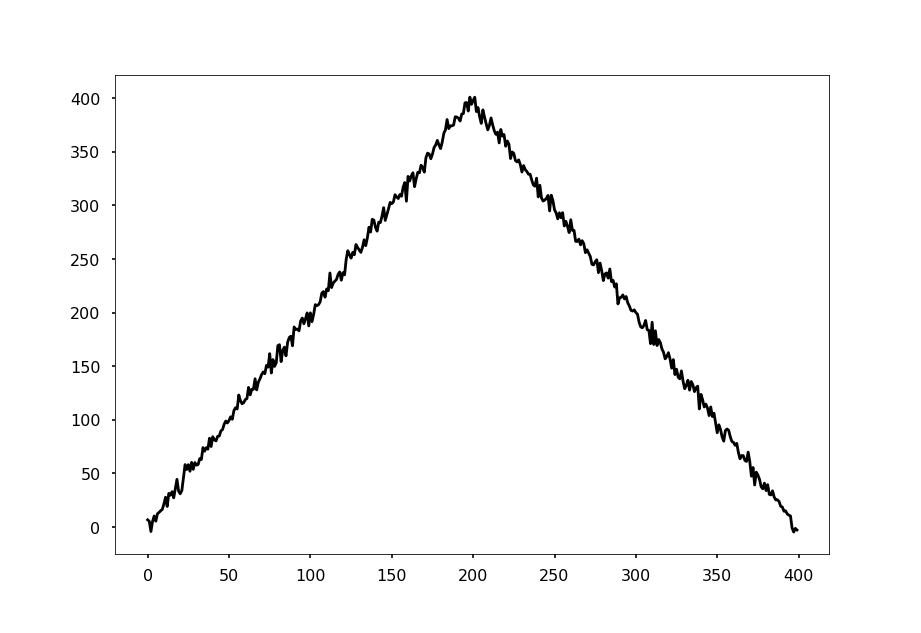
\includegraphics[scale=0.08]{images/examples_trend}
	\end{figure}
	\end{column}
     \end{columns}
     
  \begin{columns}
      \begin{column}{0.3\textwidth}
      \centering
      Mean change
      \end{column}
      \begin{column}{0.5\textwidth}
      \begin{figure}
		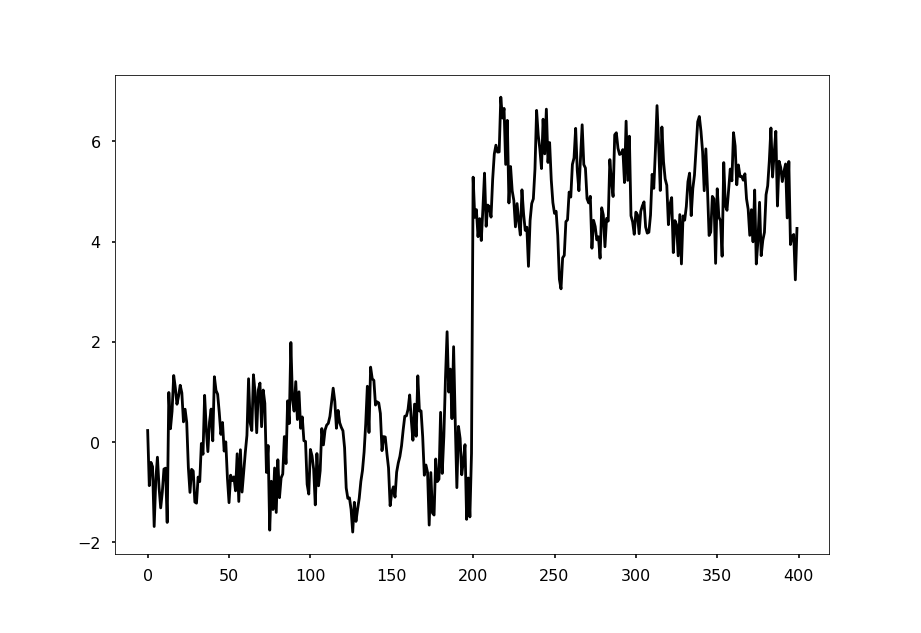
\includegraphics[scale=0.08]{images/examples_mean}
	\end{figure}
	\end{column}
     \end{columns}
     
  \begin{columns}
      \begin{column}{0.3\textwidth}
      \centering
      Variance change
      \end{column}
      \begin{column}{0.5\textwidth}
      \begin{figure}
		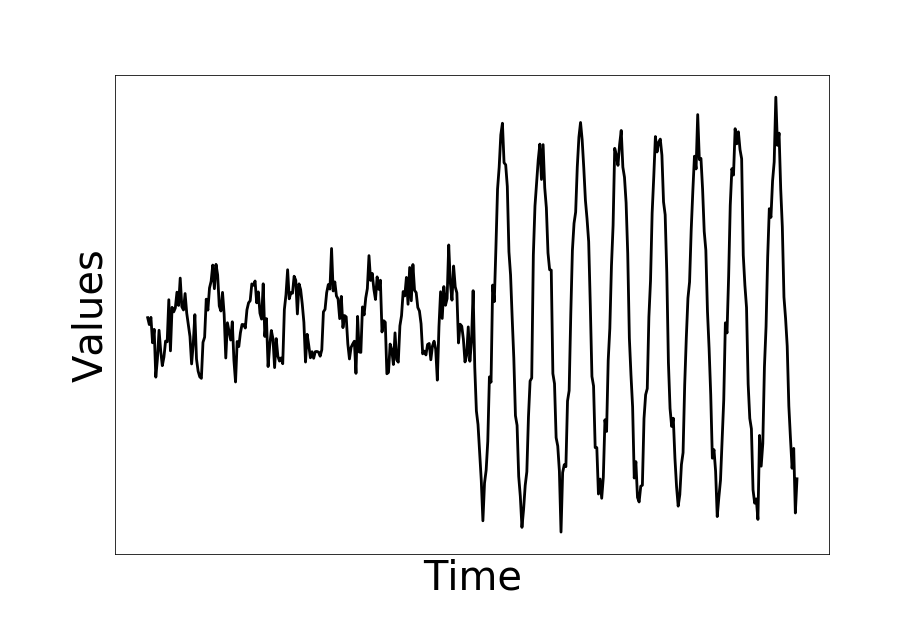
\includegraphics[scale=0.08]{images/examples_variance}
	\end{figure}
	\end{column}
     \end{columns}

	\end{column}

 \begin{column}{0.5\textwidth}
     
  \begin{columns}
      \begin{column}{0.3\textwidth}
      \centering
      Local change
      \end{column}
      \begin{column}{0.5\textwidth}
      \begin{figure}
		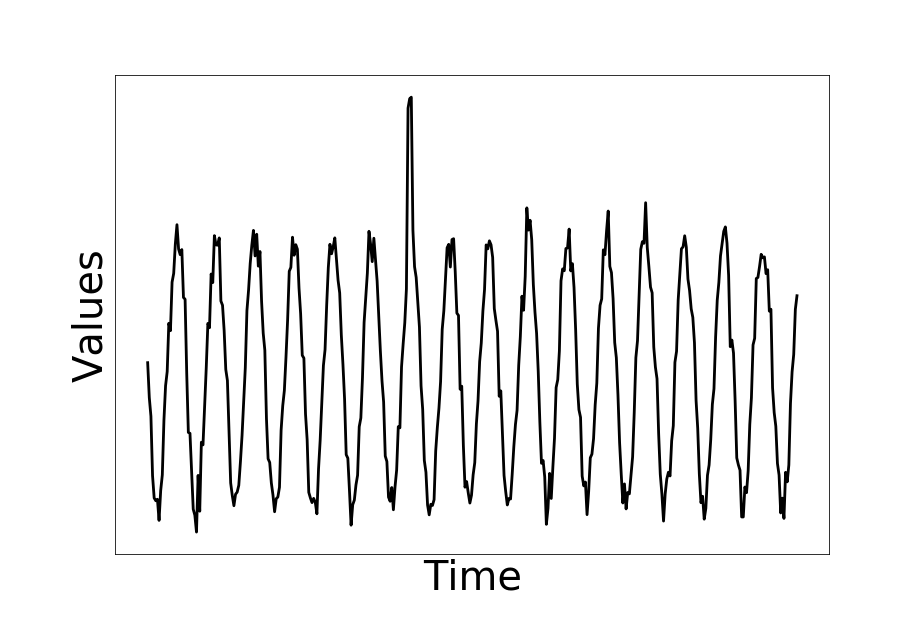
\includegraphics[scale=0.08]{images/examples_outlier}
	\end{figure}
	\end{column}
     \end{columns}
     
  \begin{columns}
      \begin{column}{0.3\textwidth}
      \centering
      Periodic component change
      \end{column}
      \begin{column}{0.5\textwidth}
      \begin{figure}
		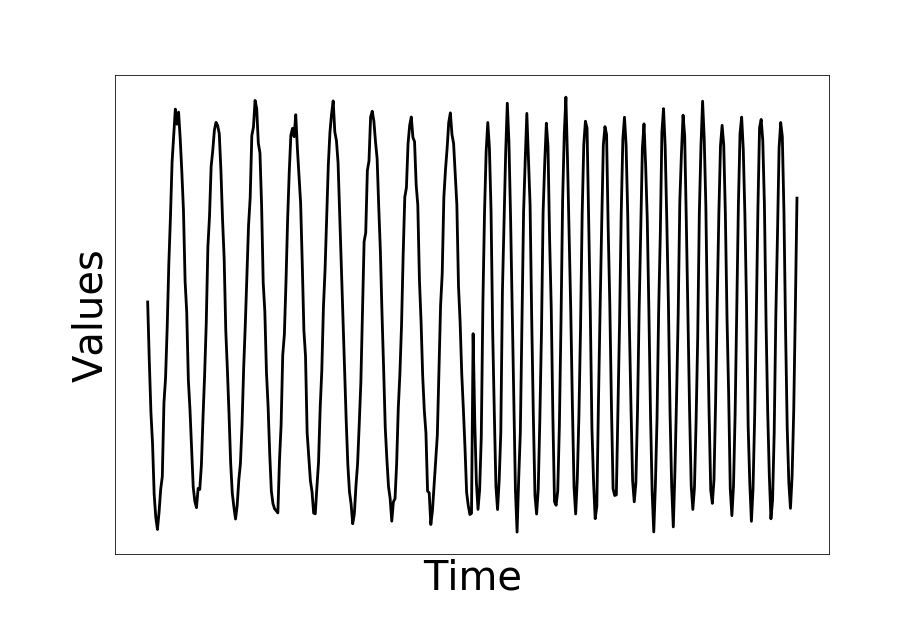
\includegraphics[scale=0.08]{images/examples_periodic}
	\end{figure}
	\end{column}
     \end{columns}

	\end{column}
	
     \end{columns}
     
\end{frame}


\section{Mobile advertising data}


\begin{frame}
\frametitle{Real data description}

   \begin{columns}
    \begin{column}{0.25\textwidth}
    \centering
     Request  
     \begin{figure}
	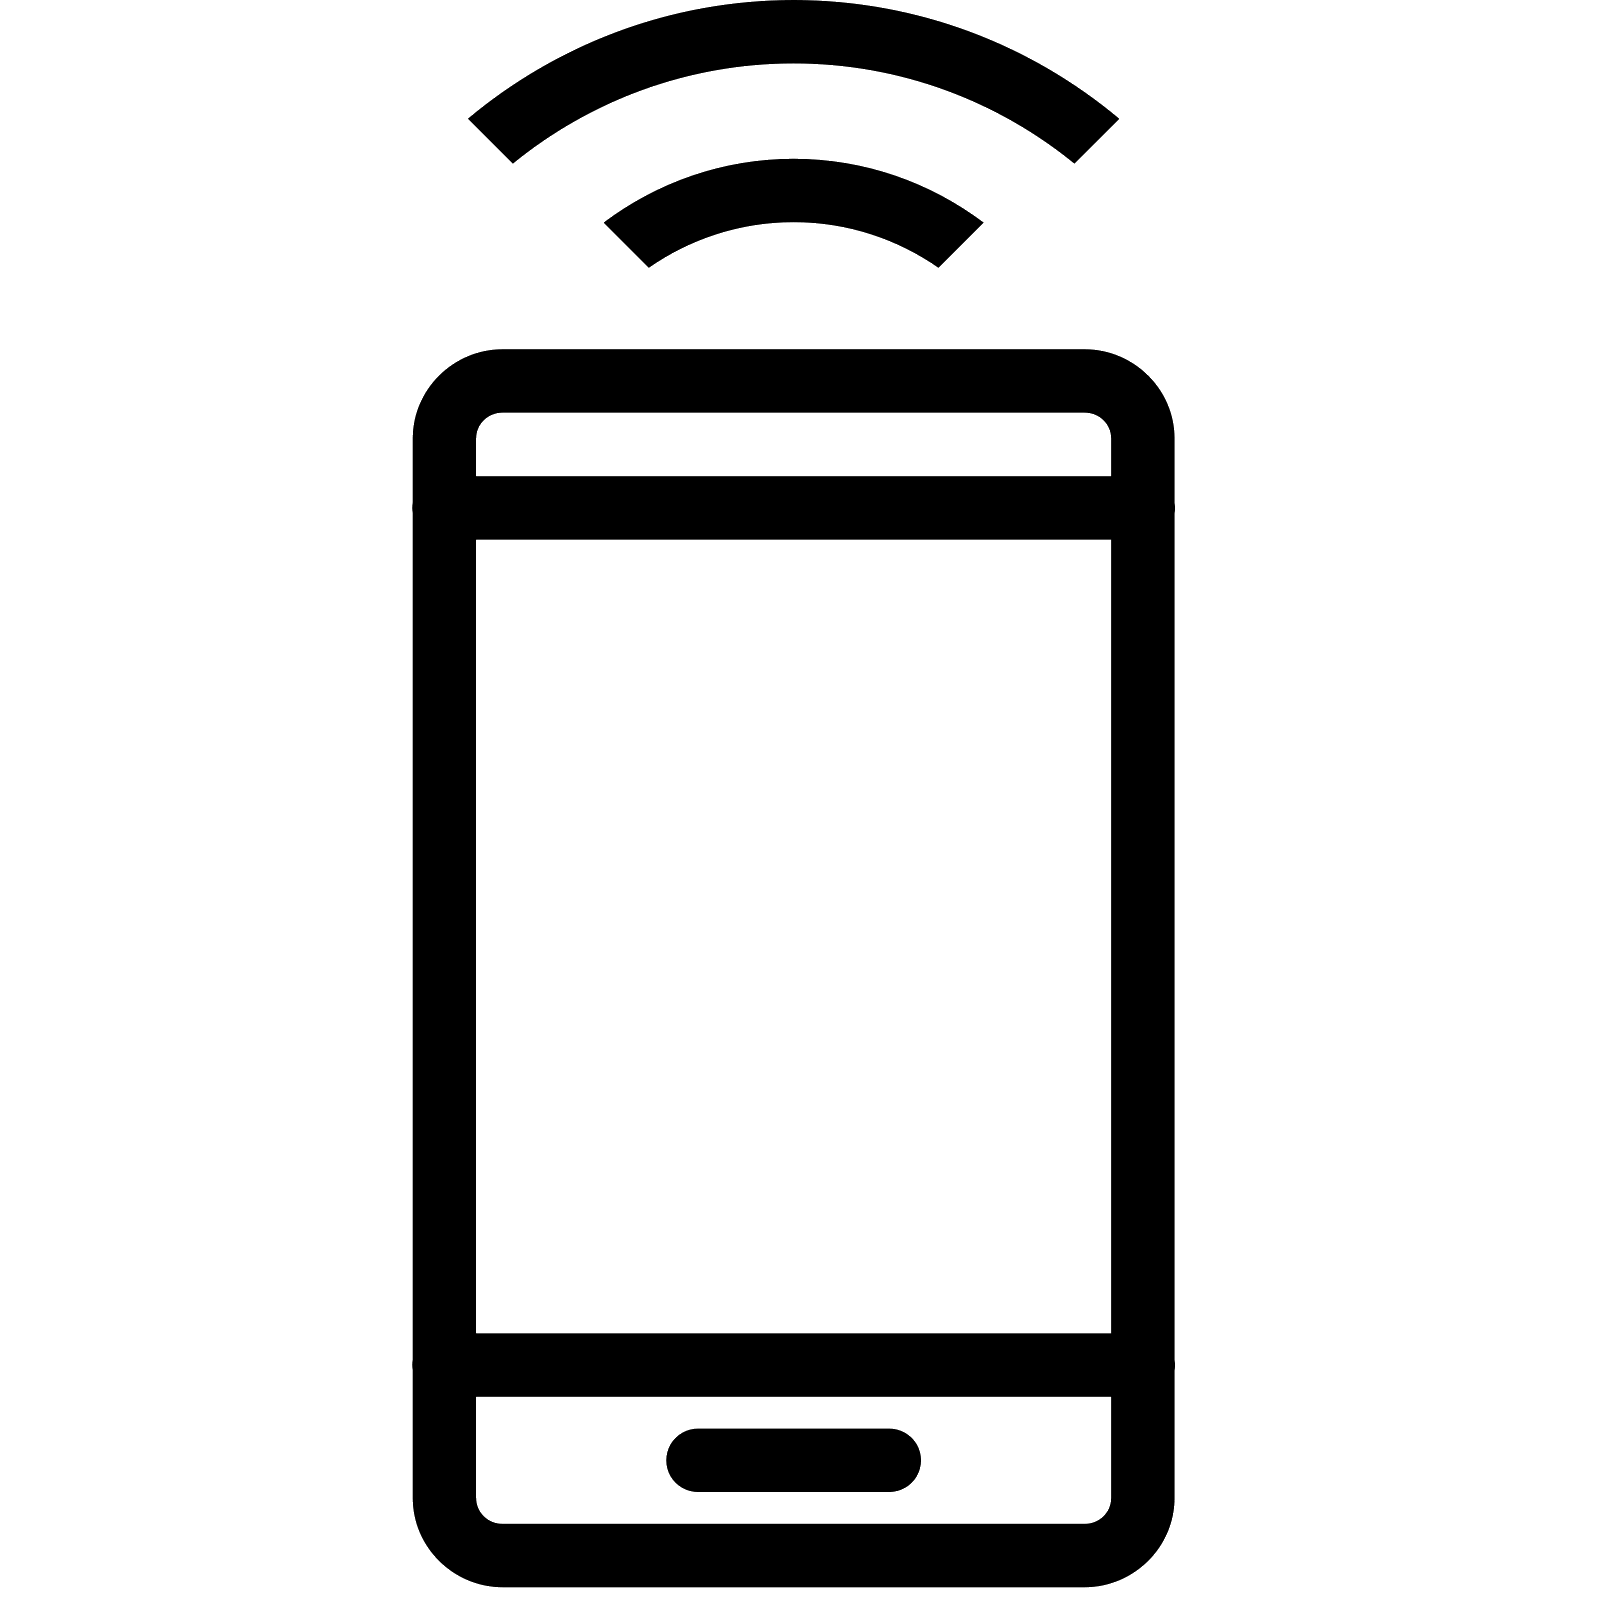
\includegraphics[height=1cm]{images/scheme_request}
     \end{figure}
     \end{column}
    \begin{column}{0.001\textwidth}
    \centering
	>
     \end{column}
    \begin{column}{0.25\textwidth}
    \centering
    Impression  
     \begin{figure}
	
\includegraphics[height=1cm]{images/scheme_impression}
     \end{figure}
    \end{column}
    \begin{column}{0.001\textwidth}
    \centering
    >
    \end{column}
    \begin{column}{0.25\textwidth}
    \centering
    Click
     \begin{figure}
	
\includegraphics[height=1cm]{images/scheme_click}
     \end{figure}
    \end{column}
    \begin{column}{0.001\textwidth}
    \centering
    >
    \end{column}
    \begin{column}{0.25\textwidth}
    \centering
     Conversion
     \begin{figure}
	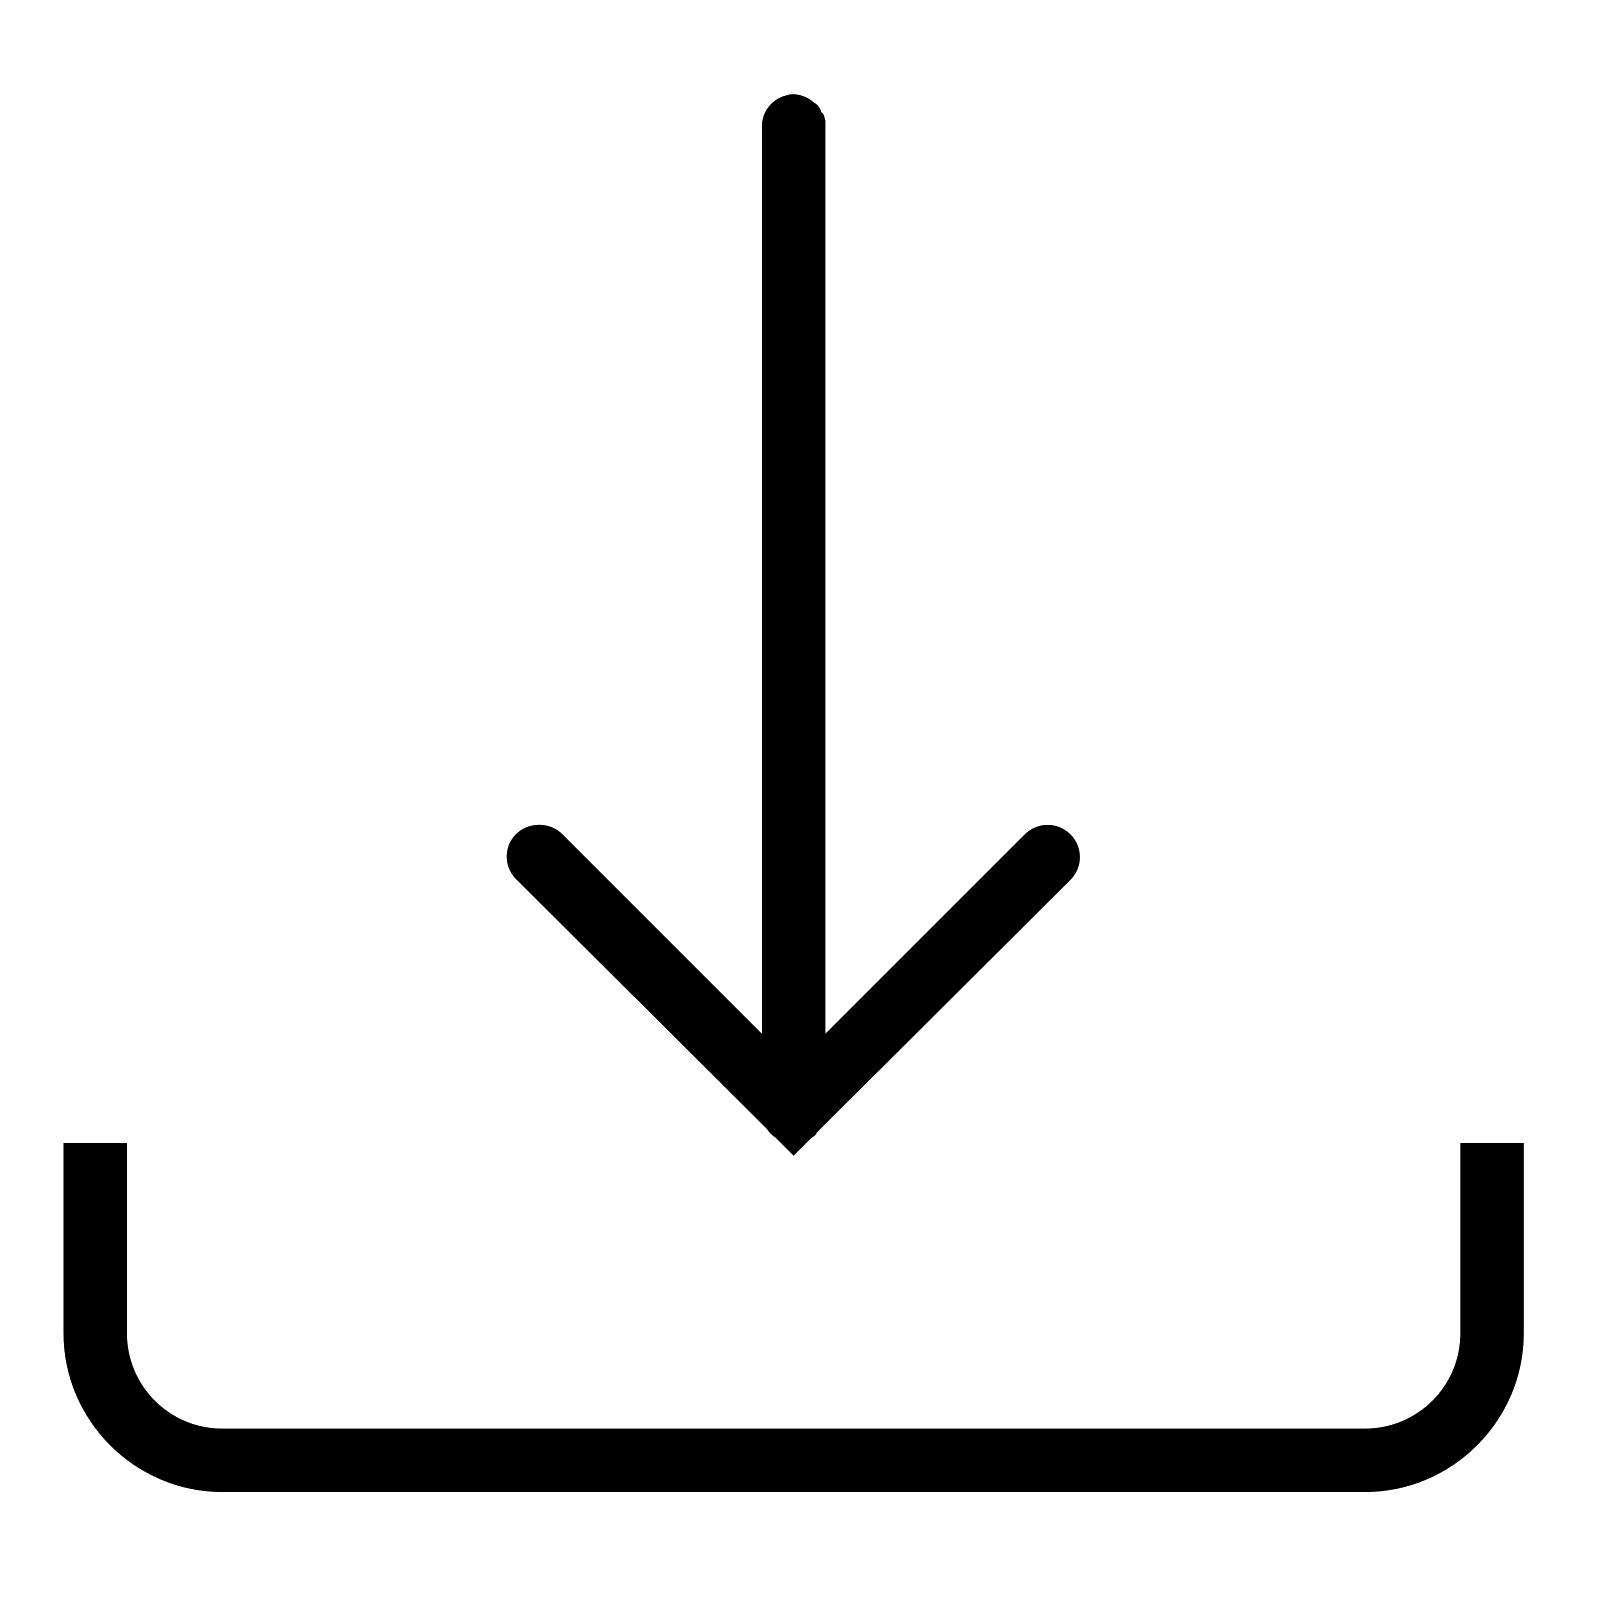
\includegraphics[height=1cm]{images/scheme_conversion}
     \end{figure}     
     \end{column}
     \end{columns}

   \begin{columns}
    \begin{column}{0.5\textwidth}
	\begin{figure}
	\textbf{Typical day}\par\medskip
	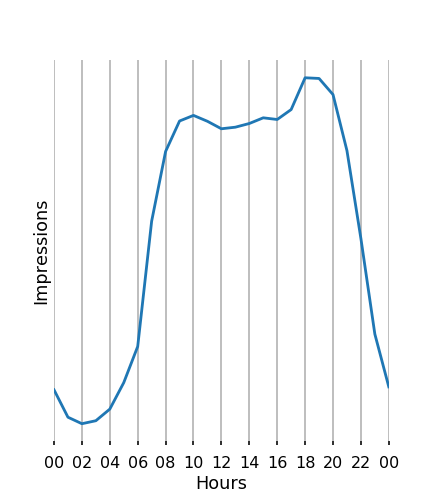
\includegraphics[height=4.5cm]{images/examples_day}
	\end{figure}
     \end{column}
    \begin{column}{0.5\textwidth}
	\begin{figure}
	\textbf{Typical weekend}\par\medskip
	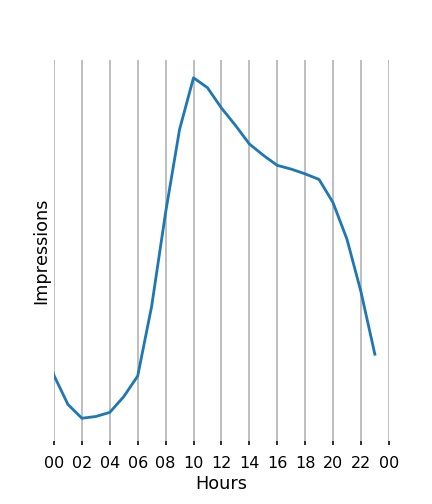
\includegraphics[height=4.5cm]{images/examples_weekend}
	\end{figure}
     \end{column}
     \end{columns}

\end{frame}

\begin{frame}
\frametitle{Real data example}
\begin{figure}
\textbf{Typical hourly impressions}\par\medskip
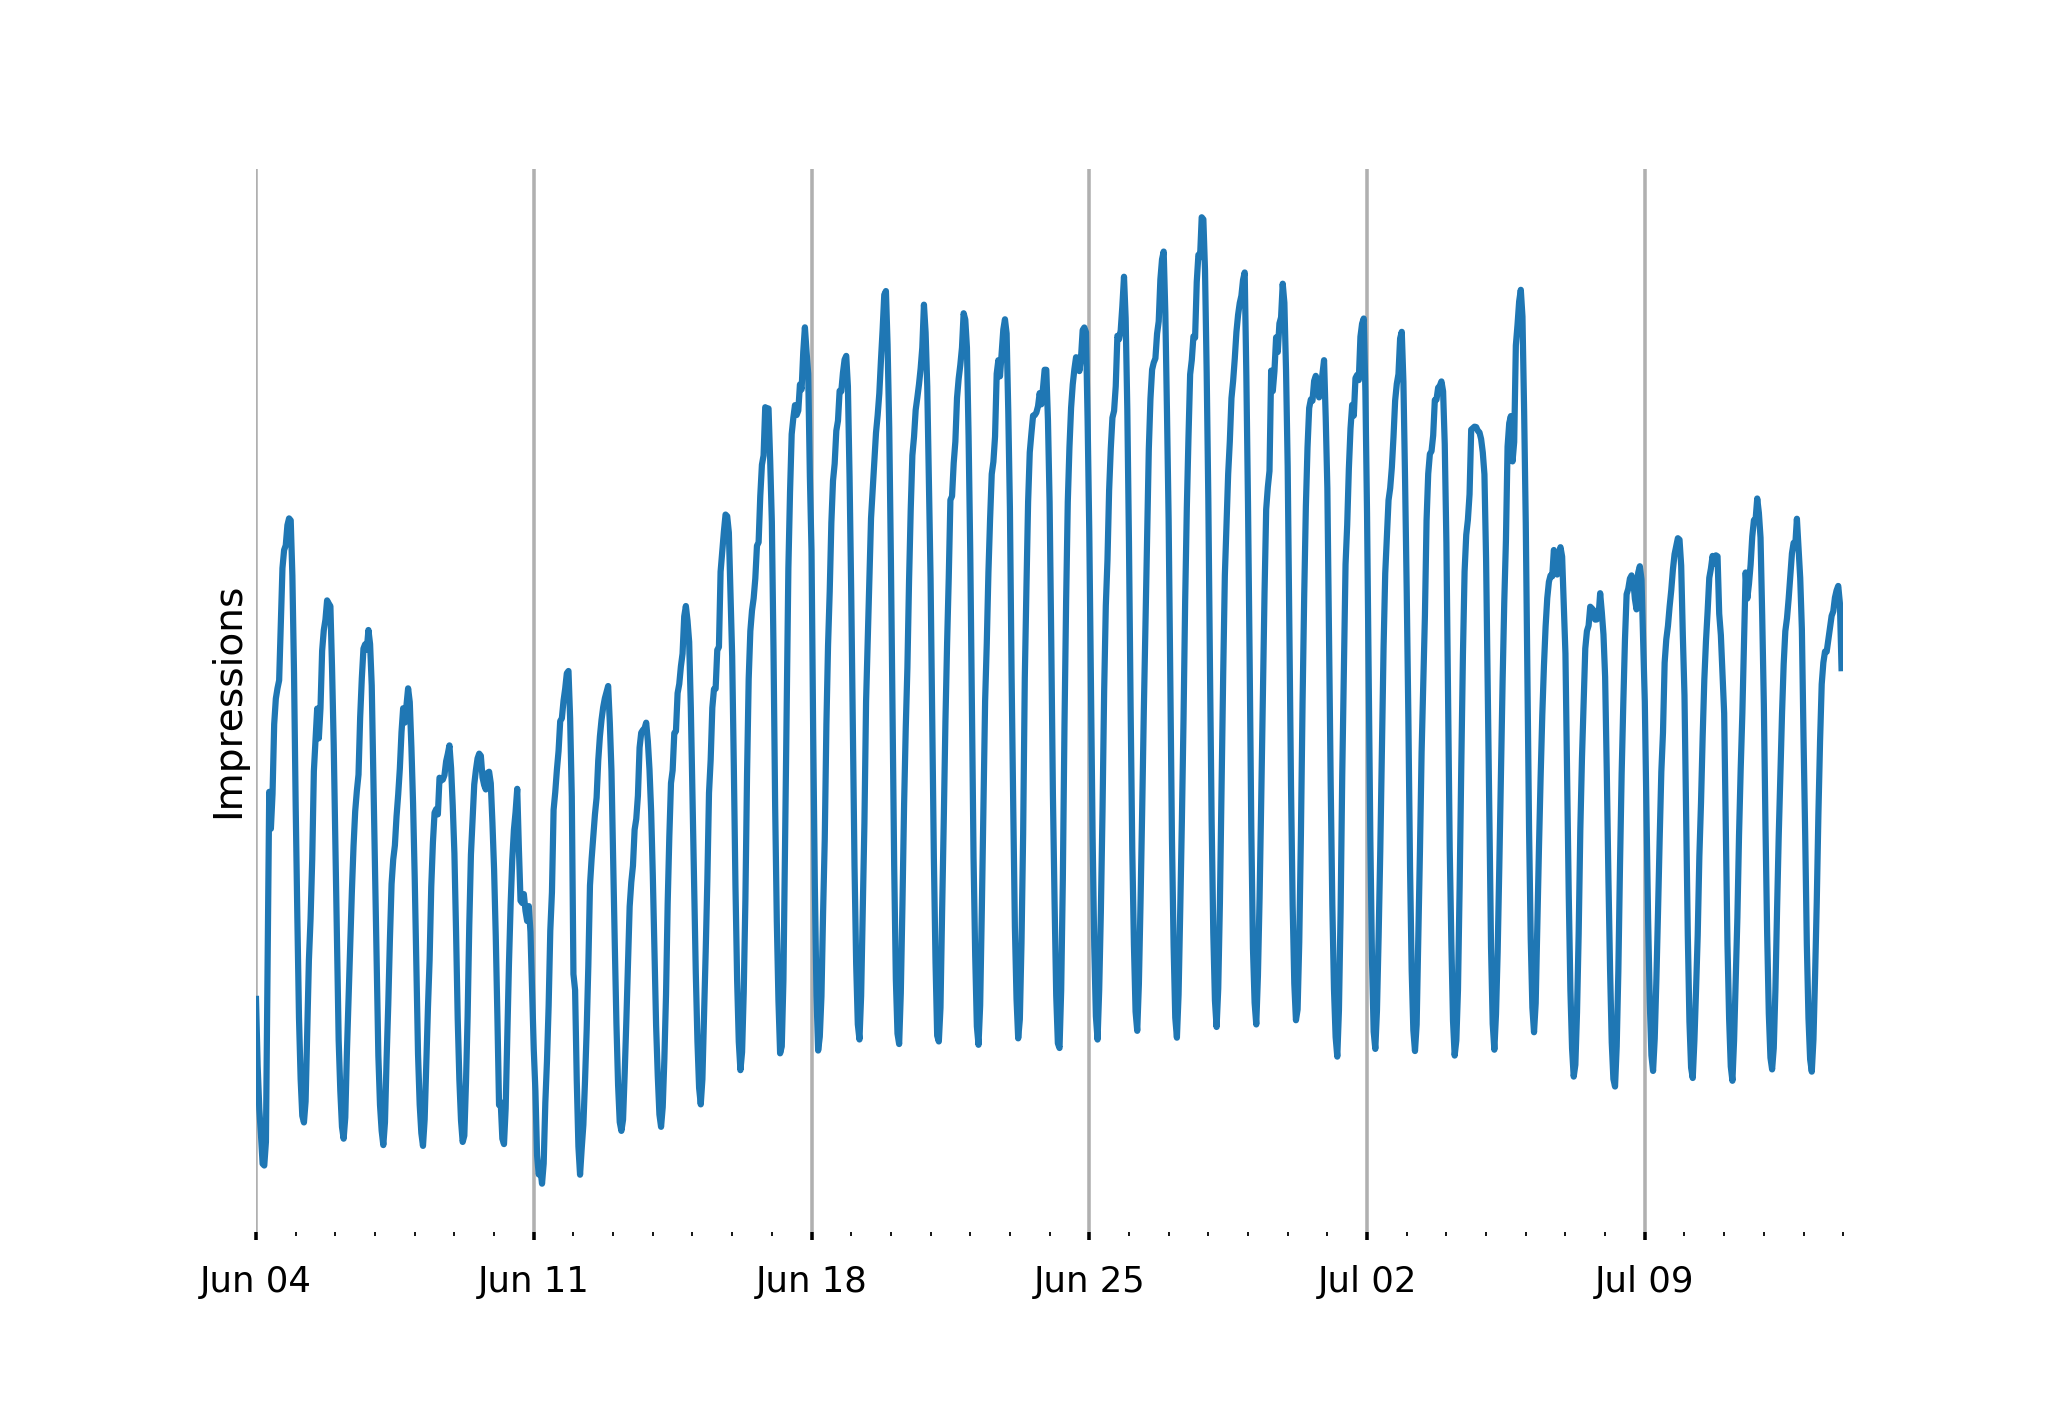
\includegraphics[scale=0.30]{images/examples_month}
\end{figure}
\end{frame}

\begin{frame}
\frametitle{Real data example}
\begin{figure}
\textbf{Typical hourly impressions}\par\medskip
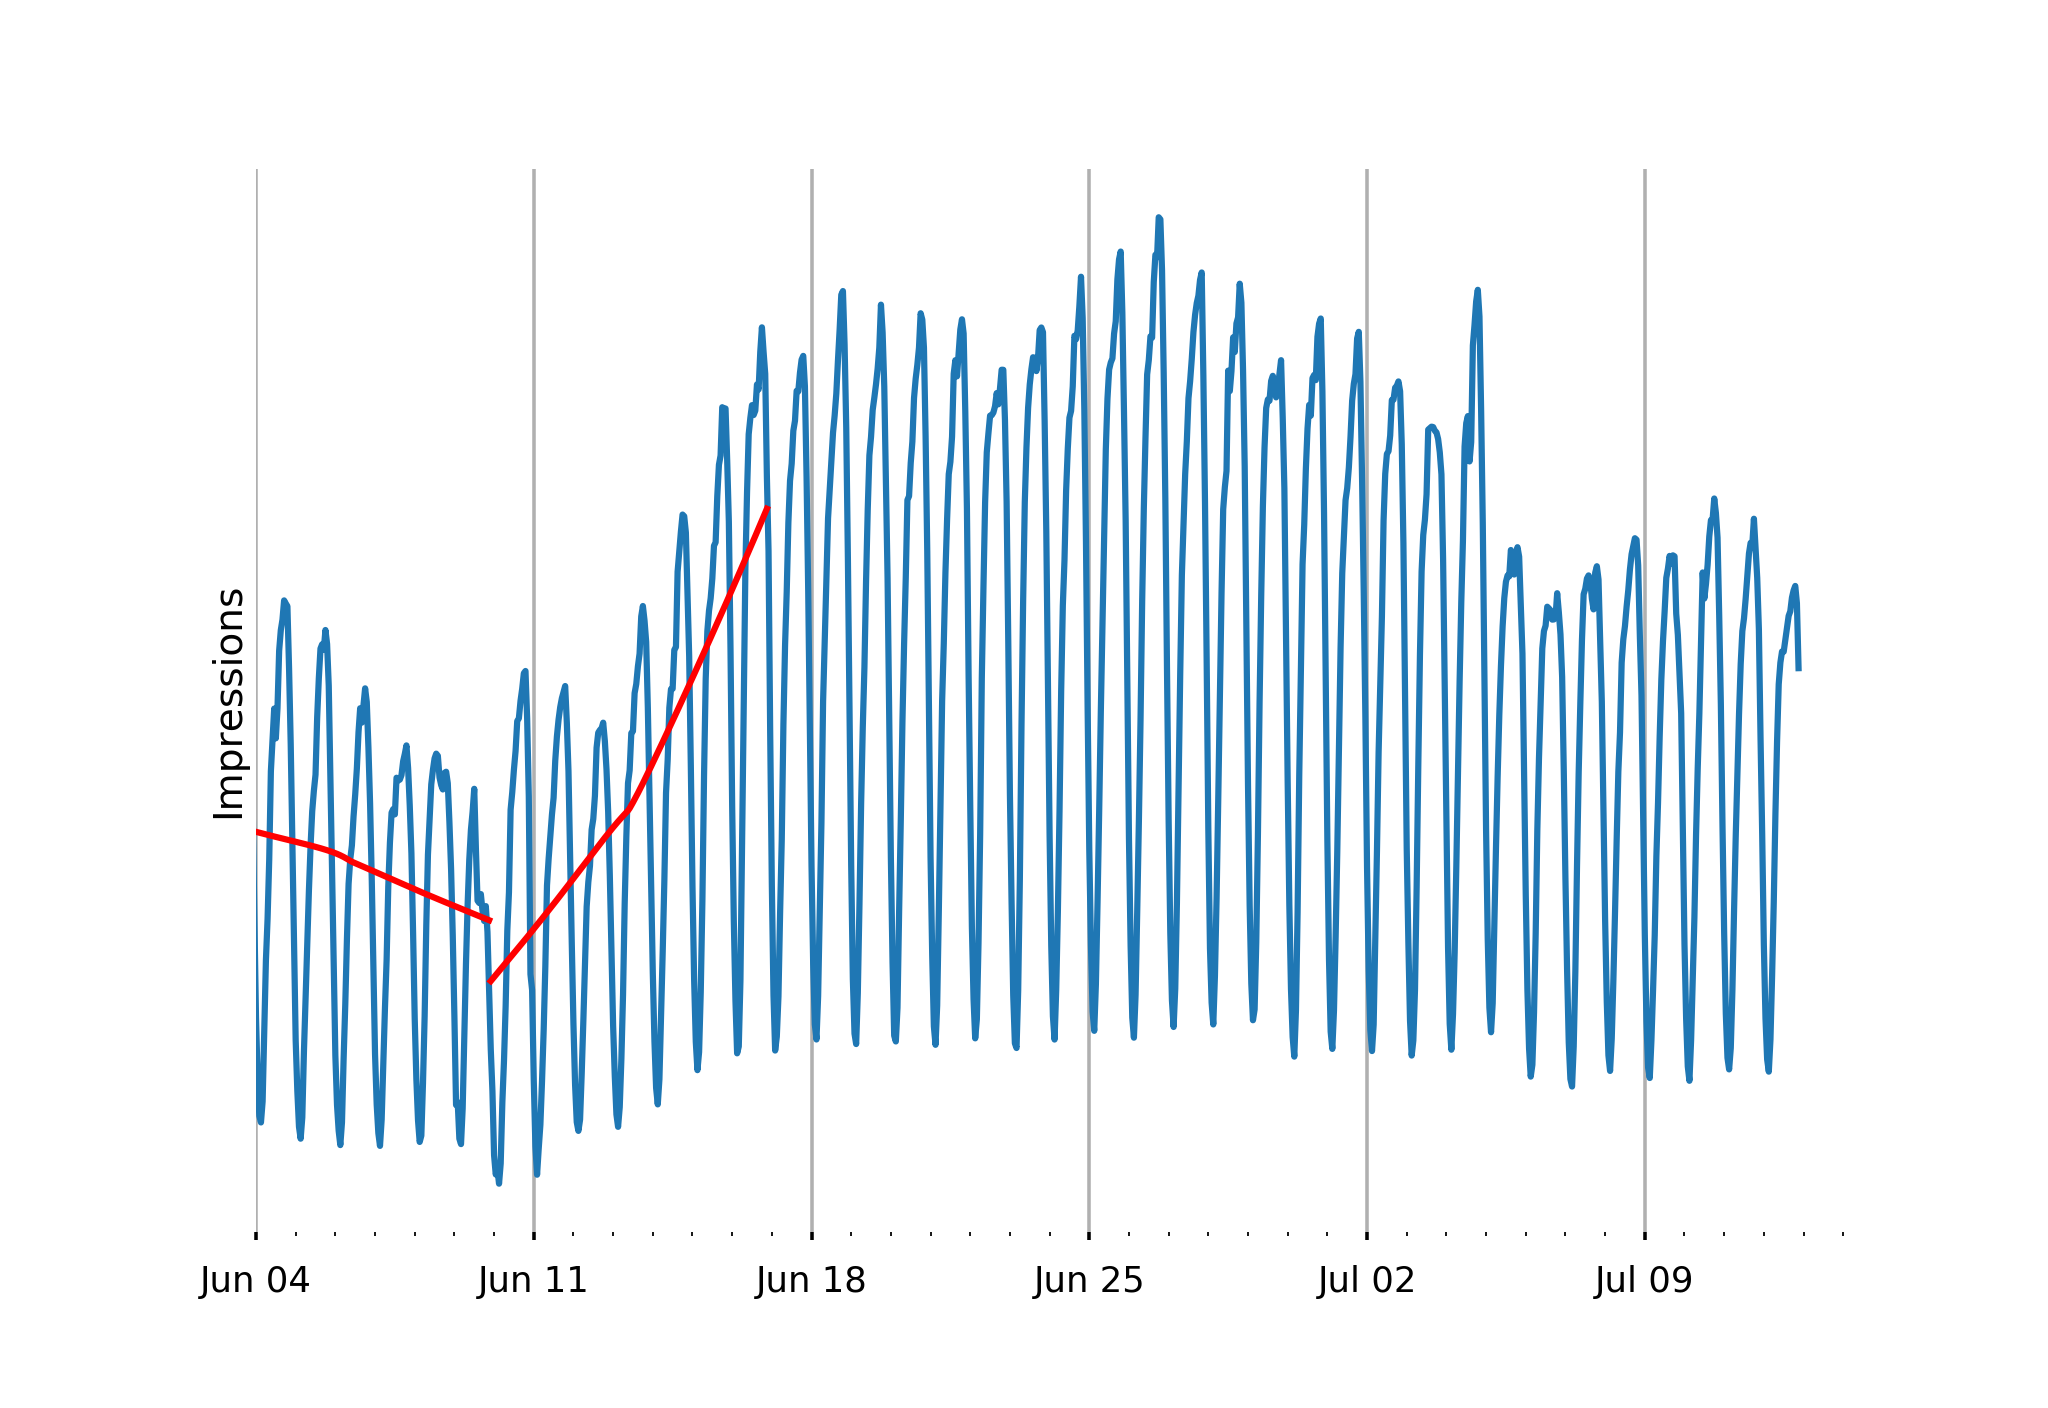
\includegraphics[scale=0.30]{images/examples_month_2}
\end{figure}
\end{frame}

\begin{frame}
\frametitle{Real data example}
\begin{figure}
\textbf{Typical hourly impressions}\par\medskip
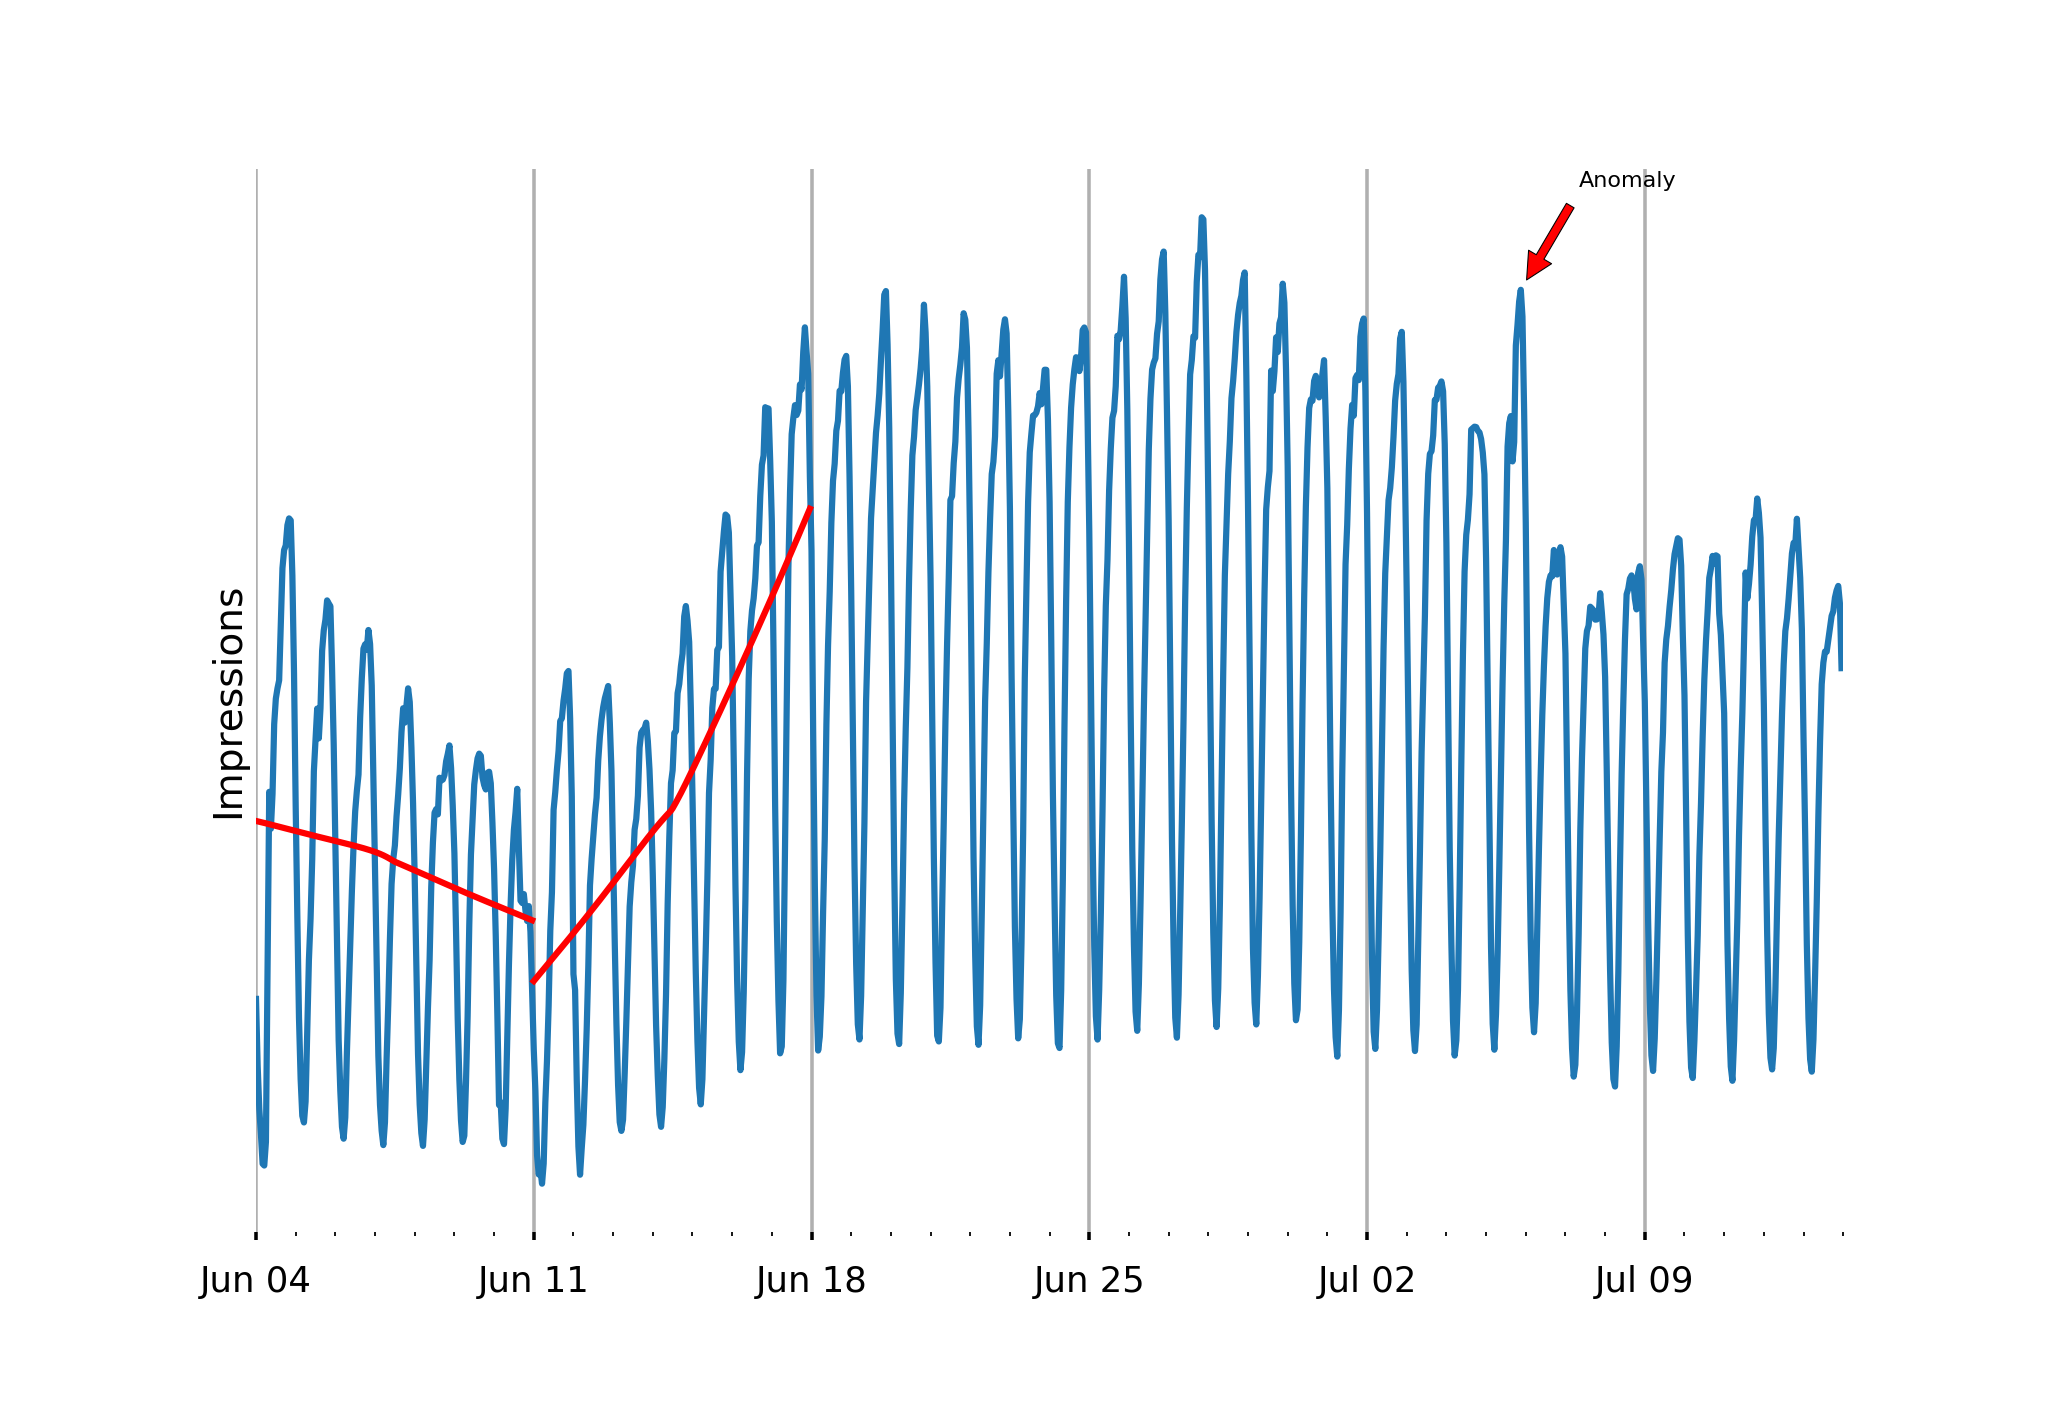
\includegraphics[scale=0.30]{images/examples_month_3}
\end{figure}
\end{frame}

\begin{frame}
\frametitle{Change point examples}
\begin{figure}
\textbf{Mean change}\par\medskip
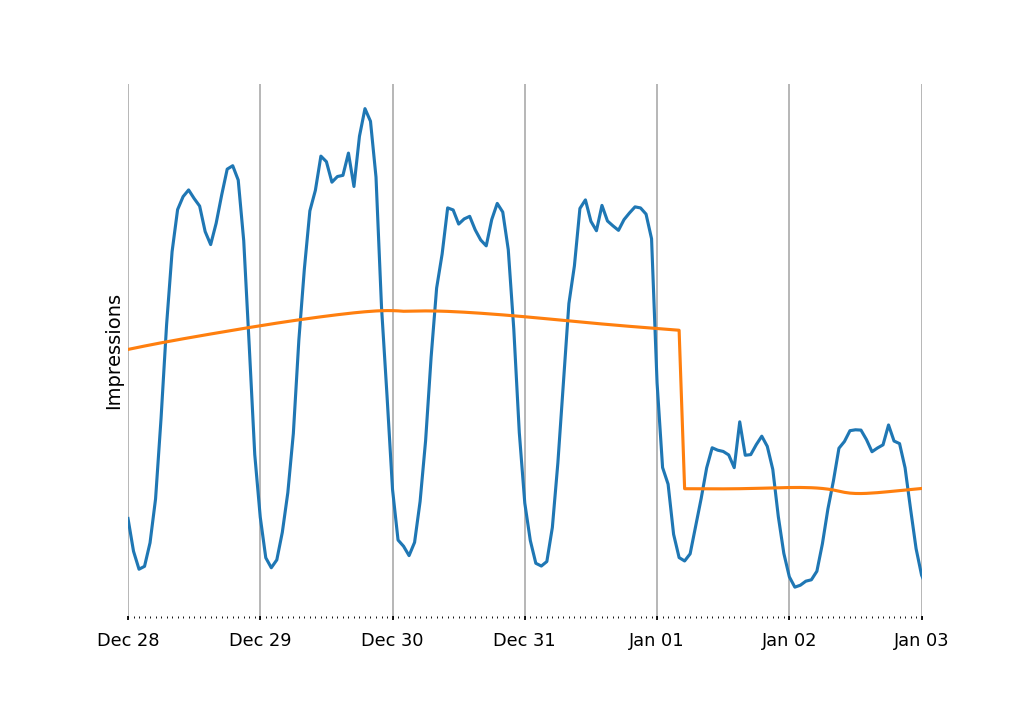
\includegraphics[scale=0.30]{images/1_examples_mean}
\end{figure}
\end{frame}


\begin{frame}
\frametitle{Change point examples}
\begin{figure}
\textbf{Local change (outlier)}\par\medskip
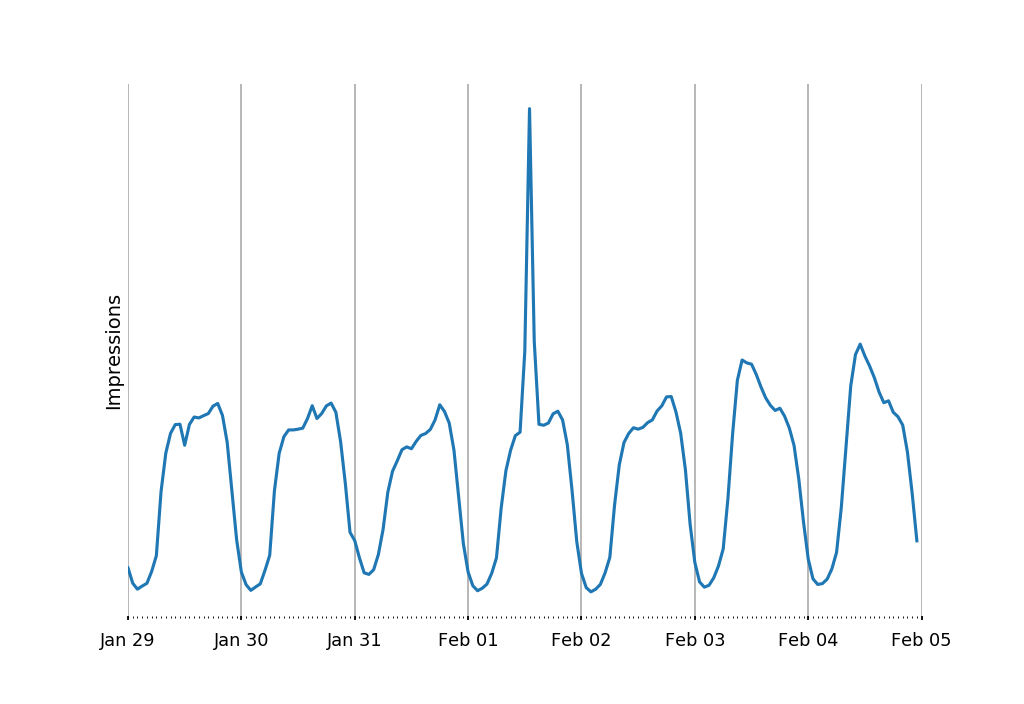
\includegraphics[scale=0.30]{images/005_point}
\end{figure}
\end{frame}

\begin{frame}
\frametitle{Change point examples}
\begin{figure}
\textbf{Periodic component change}\par\medskip
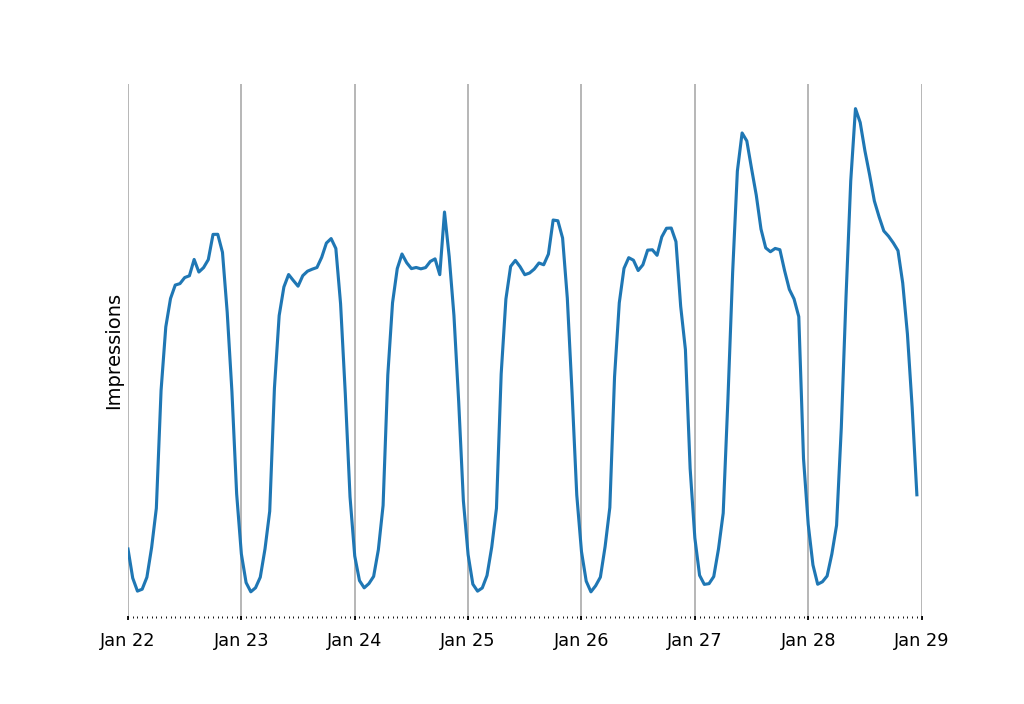
\includegraphics[scale=0.30]{images/006_structure}
\end{figure}
\end{frame}


\section{Change point detection techniques}


%\begin{frame}
  %  \frametitle{Methods}



%  \begin{columns}[T,onlytextwidth]
  %    \column{0.5\textwidth}
    %  Naïve approach 
    %\begin{itemize}
    %	\item Calculate \% difference with previous period
%	\item Compare difference with threshold
  %  \end{itemize}

%     \end{columns}

%\end{frame}

% \begin{frame}
%    \frametitle{General framework description}
%
% 	    \begin{itemize}
% 		\item Algorithm:
% 		\begin{itemize}
% 			\item Cost value is calculated for sliding windows of time series
% 			\item Cost value represents how different our model from actual data
% 			\item Once cost value more than threshold - algorithm detects change point
% 		\end{itemize}
% 		\item Types:
% 		\begin{itemize}
% 			\item Prediction based
% 			\item Approximation based
% 		\end{itemize}
% 	    	\item Input:
% 		\begin{itemize}
% 			\item Window size
% 			\item Model
% 			\item Cost function
% 			\item Threshold
% 			\item Search method
% 		\end{itemize}
% 	    \end{itemize}

% \end{frame}


\begin{frame}
    \frametitle{General framework description}

	    \begin{itemize}
		\item Preliminaries:
		\begin{itemize}
			\item Time series has structure
			\item Structure can be described by model
		\end{itemize}
		\item Idea:
		\begin{itemize}
			\item Around CP, model describes time series worse
			\item We can calculate this "worseness" using cost function
			\item Once cost value more than threshold - algorithm detects change point
		\end{itemize}
		\item Types:
		\begin{itemize}
			\item Prediction based
			\item Approximation based
		\end{itemize}
	    \end{itemize}

\end{frame}



\begin{frame}
    \frametitle{Prediction approach}

  \begin{columns}[T,onlytextwidth]
      \column{0.5\textwidth}
	\textbf{Prediction based approach}
	    \begin{itemize}
	    	\item Predict with appropriate model
		\item Calculate difference between prediction and actual data (with appropriate cost function)
		\item Compare difference with threshold
	    \end{itemize}
      \column{0.5\textwidth}
      Example: change in mean
      \begin{figure}
	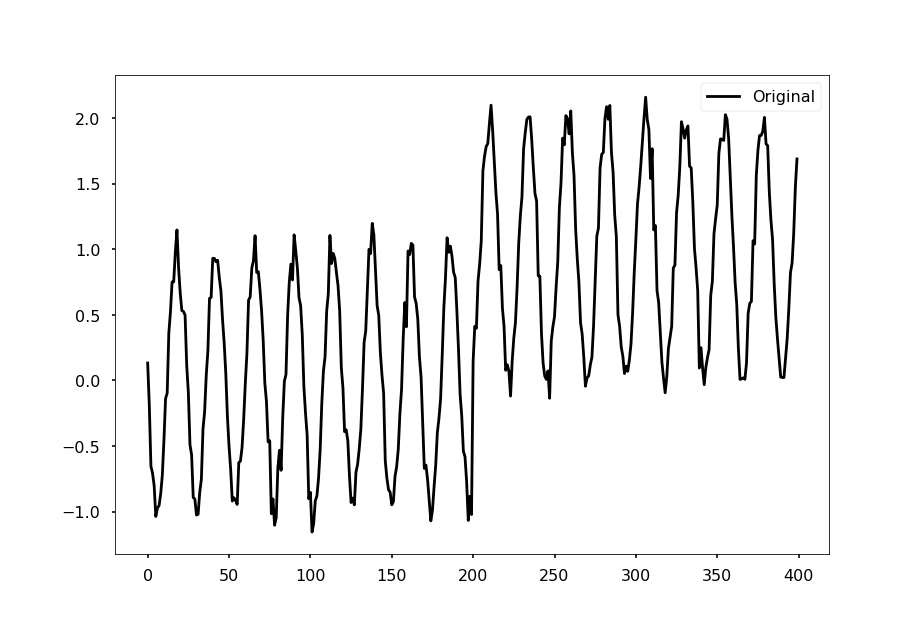
\includegraphics[scale=0.2]{images/approaches_first_1}
	\end{figure}
     \end{columns}

\end{frame}

\begin{frame}
    \frametitle{Prediction approach}
  \begin{columns}[T,onlytextwidth]
      \column{0.5\textwidth}
	Prediction based approach
	    \begin{itemize}
	    	\item Predict with appropriate model
		\item Calculate difference between prediction and actual data (with appropriate cost function)
		\item Compare difference with threshold
	    \end{itemize}
      \column{0.5\textwidth}
      Example: change in mean; model is a constant trend
      \begin{figure}
	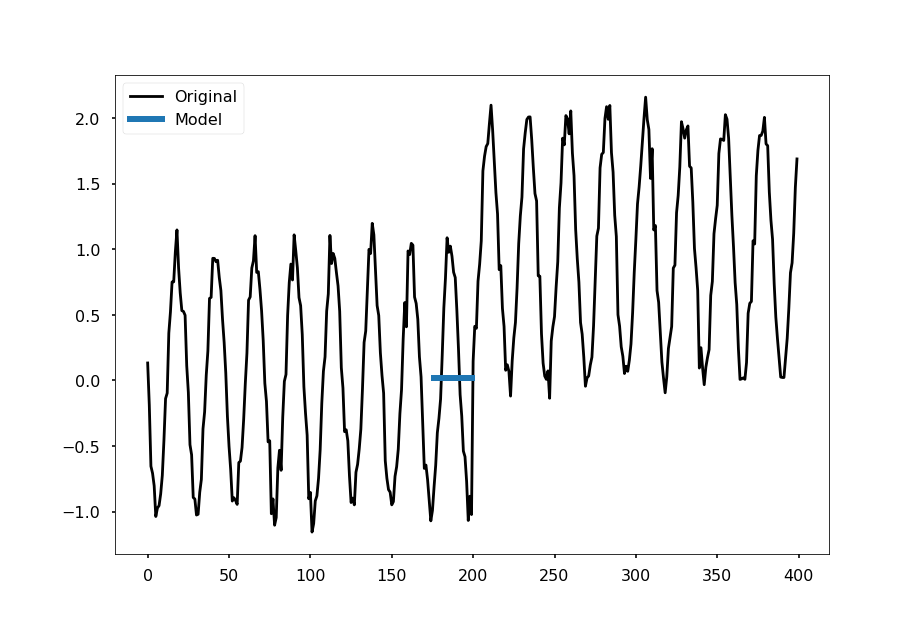
\includegraphics[scale=0.2]{images/approaches_first_2}
	\end{figure}
     \end{columns}
\end{frame}

\begin{frame}
    \frametitle{Prediction approach}
  \begin{columns}[T,onlytextwidth]
      \column{0.5\textwidth}
	Prediction based approach
	    \begin{itemize}
	    	\item Predict with appropriate model
		\item Calculate difference between prediction and actual data (with appropriate cost function)
		\item Compare difference with threshold
	    \end{itemize}
      \column{0.5\textwidth}
      Example: change in mean; model is a constant trend
      \begin{figure}
	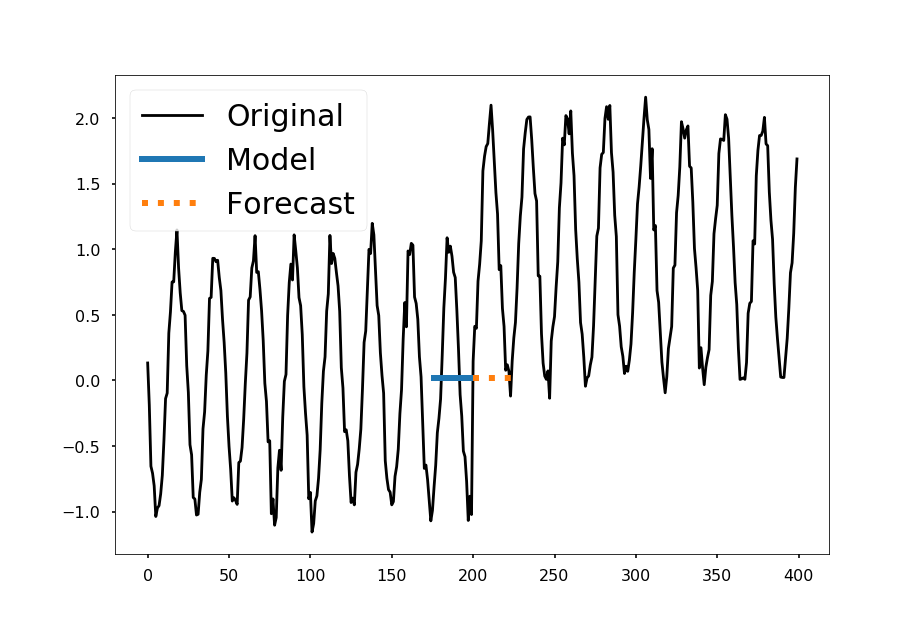
\includegraphics[scale=0.2]{images/approaches_first_3}
	\end{figure}
     \end{columns}
\end{frame}

\begin{frame}
    \frametitle{Prediction approach}
  \begin{columns}[T,onlytextwidth]
      \column{0.5\textwidth}
	Prediction based approach
	    \begin{itemize}
	    	\item Predict with appropriate model
		\item Calculate difference between prediction and actual data (with appropriate cost function)
		\item Compare difference with threshold
	    \end{itemize}
      \column{0.5\textwidth}
      Example: change in mean; model is a constant trend
      \begin{figure}
	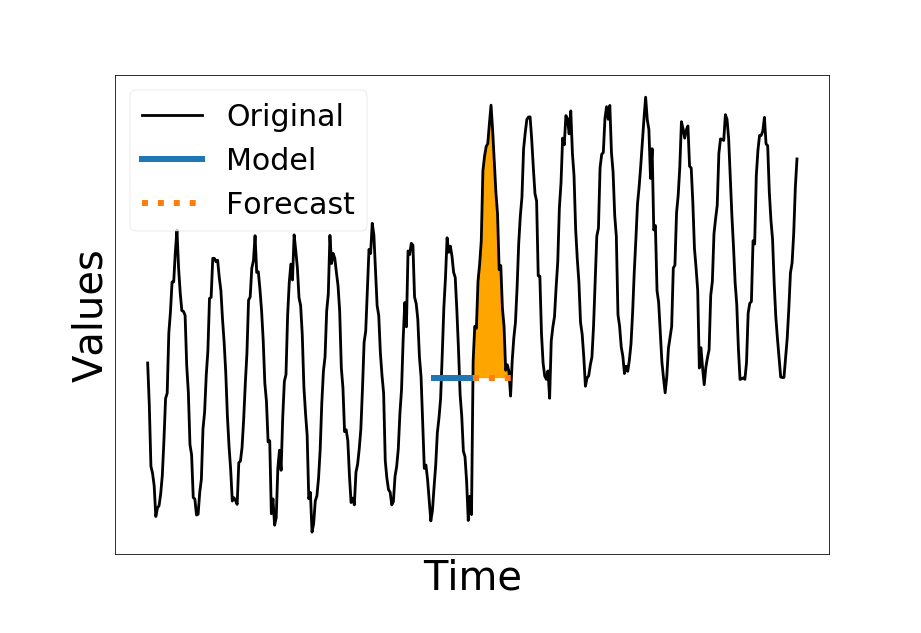
\includegraphics[scale=0.2]{images/approaches_first_4}
	\end{figure}
     \end{columns}
\end{frame}

\begin{frame}
    \frametitle{Prediction approach}
  \begin{columns}[T,onlytextwidth]
      \column{0.5\textwidth}
	Prediction based approach
	    \begin{itemize}
	    	\item Predict with appropriate model
		\item Calculate difference between prediction and actual data (with appropriate cost function)
		\item Compare difference with threshold
	    \end{itemize}
      \column{0.5\textwidth}
      Example: change in mean; model is a constant trend
      \begin{figure}
	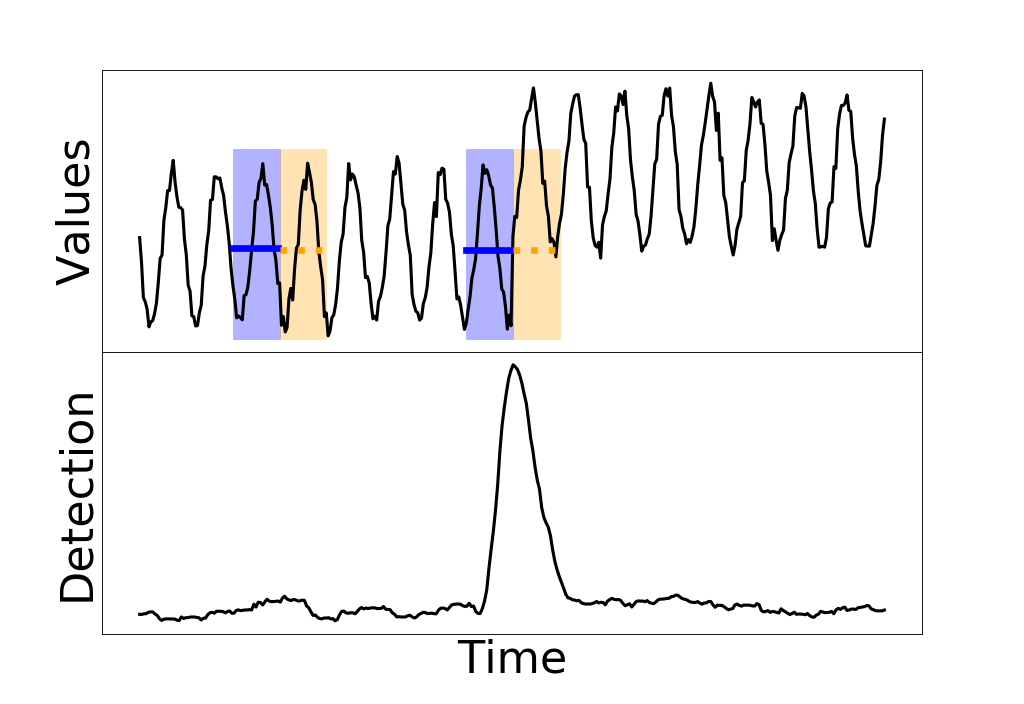
\includegraphics[scale=0.2]{images/approaches_first_5}
	\end{figure}
     \end{columns}
\end{frame}


\begin{frame}
    \frametitle{Approximation approach}

  \begin{columns}[T,onlytextwidth]
      \column{0.5\textwidth}
      \textbf{Approximation based approach}
	    \begin{itemize}
	    	\item Approximate time series with appropriate model
		\item Calculate difference between overall approximation and approximation of left and right halves (with appropriate cost function)
		\item Find points to minimize difference
	    \end{itemize}
     \column{0.5\textwidth}
      Example: change in mean; model is a constant trend
      	\begin{figure}
		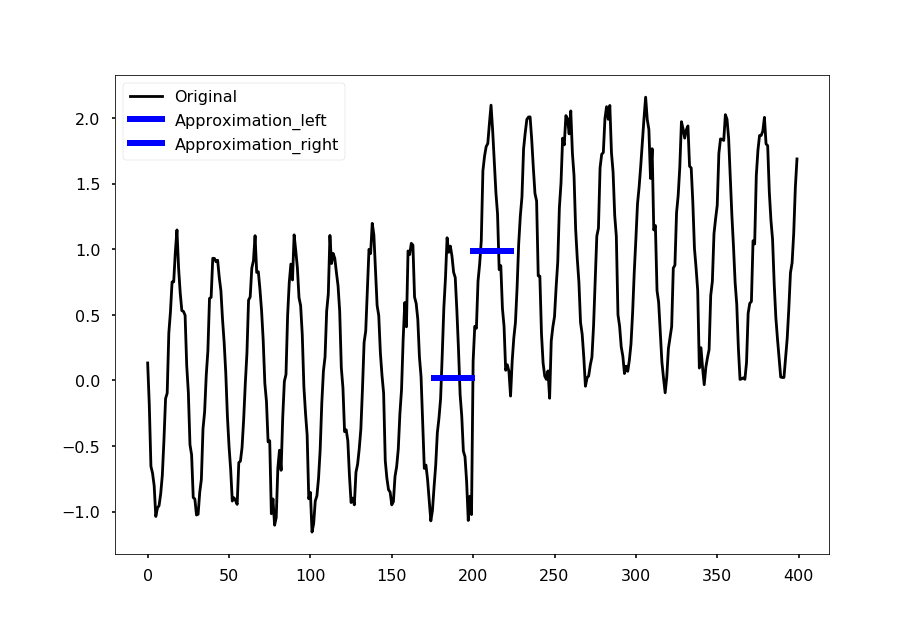
\includegraphics[scale=0.2]{images/approaches_second_1}
	\end{figure}
     \end{columns}

\end{frame}

\begin{frame}
    \frametitle{Approximation approach}
  \begin{columns}[T,onlytextwidth]
      \column{0.5\textwidth}
	Approximation based approach
	    \begin{itemize}
	    	\item Approximate time series with appropriate model
		\item Calculate difference between overall approximation and approximation of left and right halves (with appropriate cost function)
		\item Find points to minimize difference
	    \end{itemize}
     \column{0.5\textwidth}
      Example: change in mean; model is a constant trend
      	\begin{figure}
		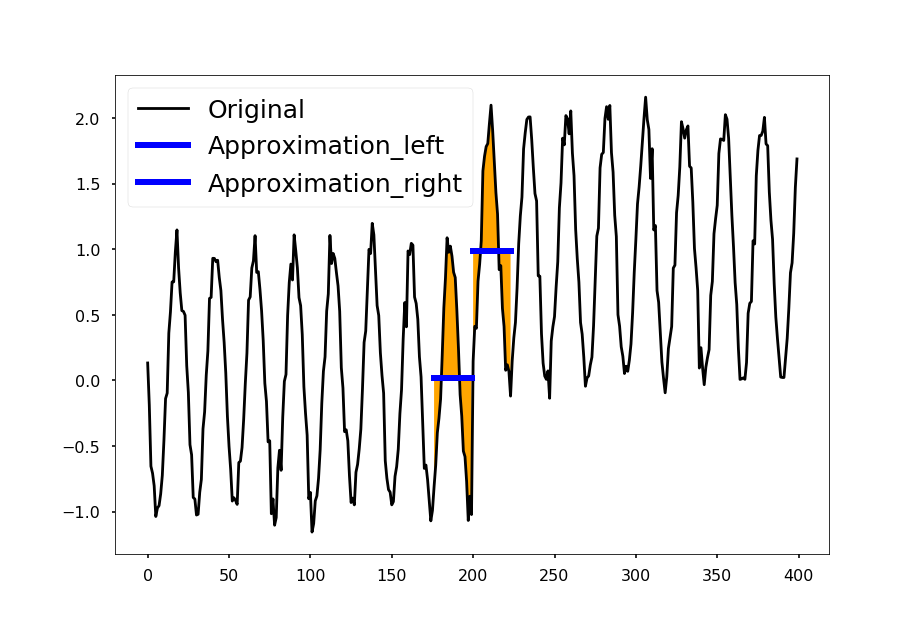
\includegraphics[scale=0.2]{images/approaches_second_2}
	\end{figure}
     \end{columns}
\end{frame}

\begin{frame}
    \frametitle{Approximation approach}
  \begin{columns}[T,onlytextwidth]
      \column{0.5\textwidth}
	Approximation based approach
	    \begin{itemize}
	    	\item Approximate time series with appropriate model
		\item Calculate difference between overall approximation and approximation of left and right halves (with appropriate cost function)
		\item Find points to minimize difference
	    \end{itemize}
     \column{0.5\textwidth}
      Example: change in mean; model is a constant trend
      	\begin{figure}
		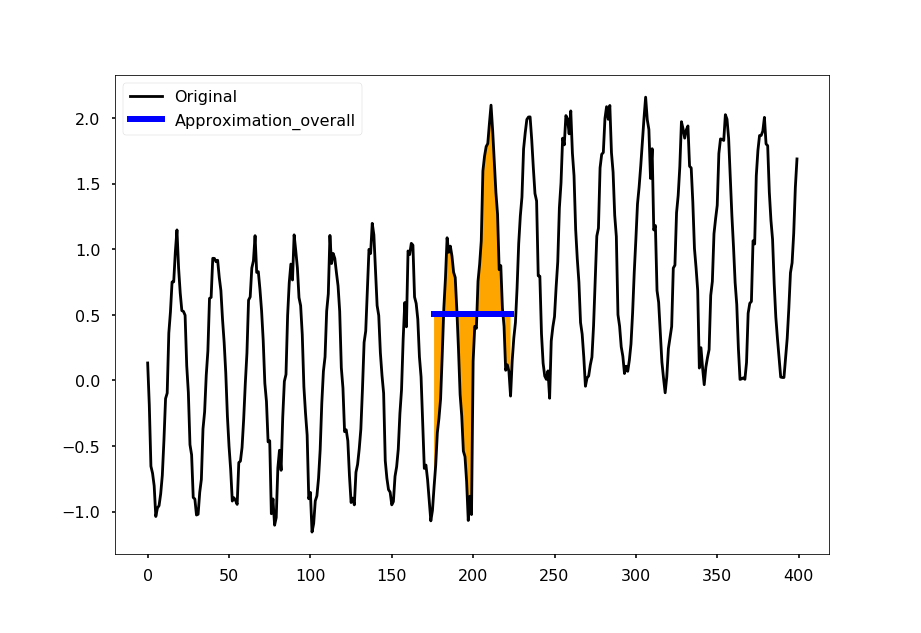
\includegraphics[scale=0.2]{images/approaches_second_3}
	\end{figure}
     \end{columns}
\end{frame}

\begin{frame}
    \frametitle{Approximation approach}
  \begin{columns}[T,onlytextwidth]
      \column{0.5\textwidth}
	Approximation based approach
	    \begin{itemize}
	    	\item Approximate time series with appropriate model
		\item Calculate difference between overall approximation and approximation of left and right halves (with appropriate cost function)
		\item Find points to minimize difference
	    \end{itemize}
     \column{0.5\textwidth}
      Example: change in mean; model is a constant trend
      	\begin{figure}
		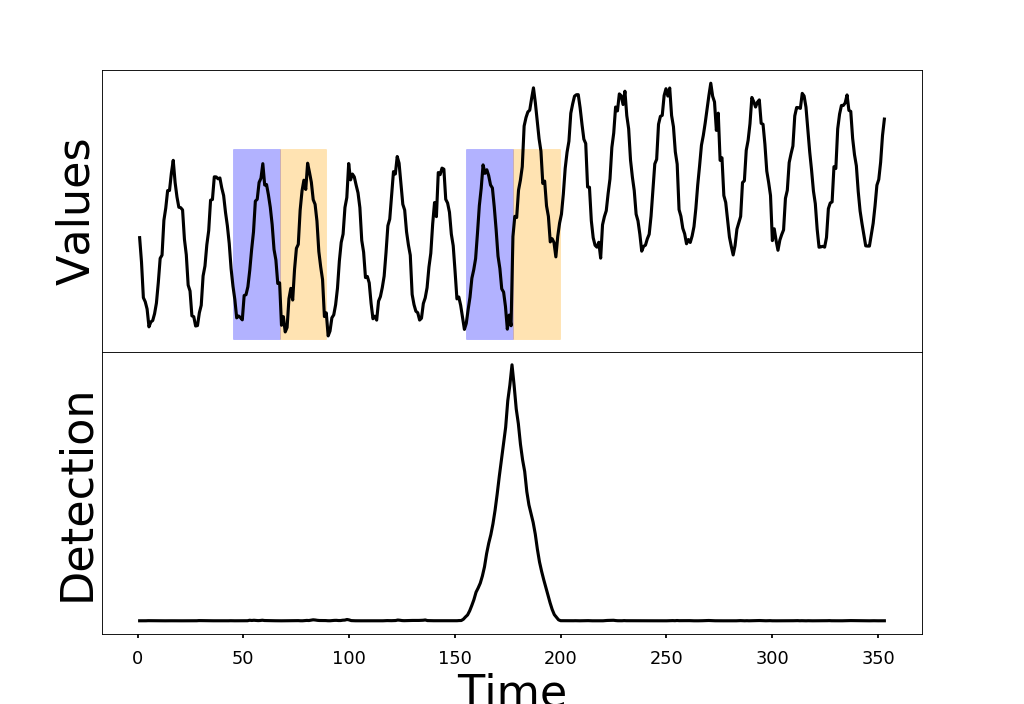
\includegraphics[scale=0.2]{images/approaches_second_4}
	\end{figure}
     \end{columns}
\end{frame}


\begin{frame}
    \frametitle{Things to define}
	 
	\begin{itemize}
	    	\item Model. Based on what changes do you want to find and specifics of your time series
			\begin{itemize}
			\item Mean - level (constant trend)
			\item Regression - trend
			\item Mean + Daily fluctuations
			\item Others
			\end{itemize}
		\item Window size. Based on time frame that is significant to your task
		\item Cost function. Based on what changes do you want to find.
		\item Threshold. Depends on small or big changes would you like to find
		\item Search method. Based on your task
	    \end{itemize}

 \end{frame}

\section{Applications to real data}



\begin{frame}
    \frametitle{Applications to real data}
 
 Let's apply these approaches to real data (described in previous section).
We have chosen two models.
Mean model as basic model which works generally good:
$$ \mathrm{X} = A + \epsilon $$
Model, which appropriate to our data nature:
$$ \mathrm{X} = a + C\cos(2\pi \frac{n}{24} + \phi) + \epsilon $$
Cost function will be mean square error
% $$ c(\mathbf{X}_I) = \sum_{t \in I}||\mathbf{X}_t - \bar{\mathbf{X}} ||_2^2 $$
Window size will be 48 points.
 
 \end{frame}



\begin{frame}
    \frametitle{Applications to real data. Mean change}
  \begin{columns}[T,onlytextwidth]
      \column{0.5\textwidth}
	\begin{figure}
	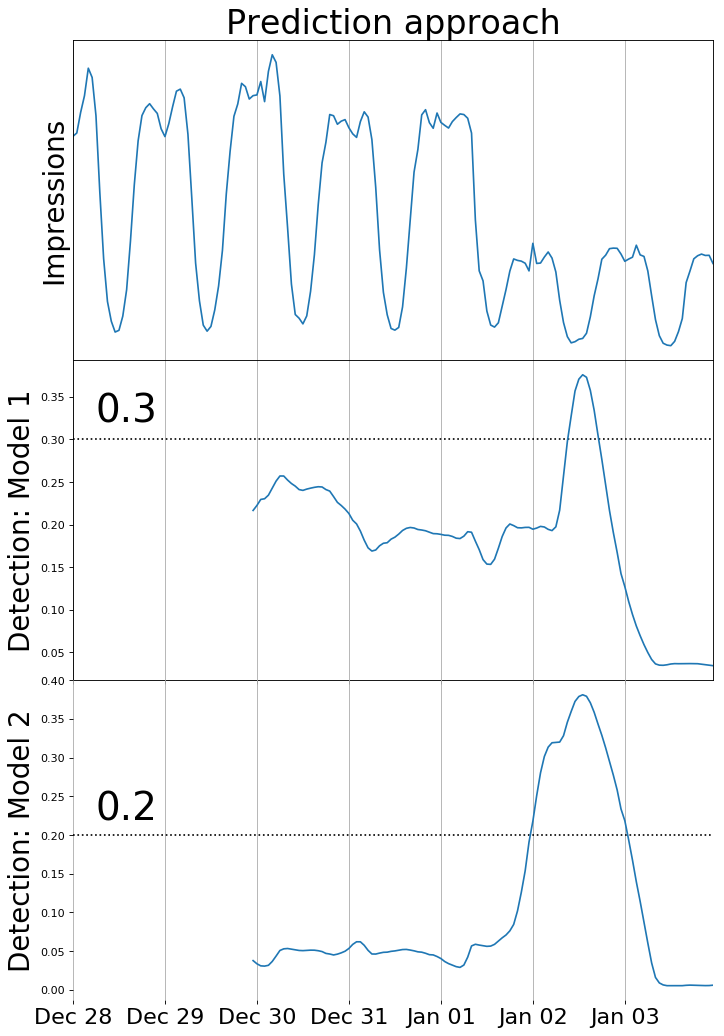
\includegraphics[height=6.5cm]{images/methods_comparison_1_1}
	\end{figure}
	
      \column{0.5\textwidth}
	\begin{figure}
	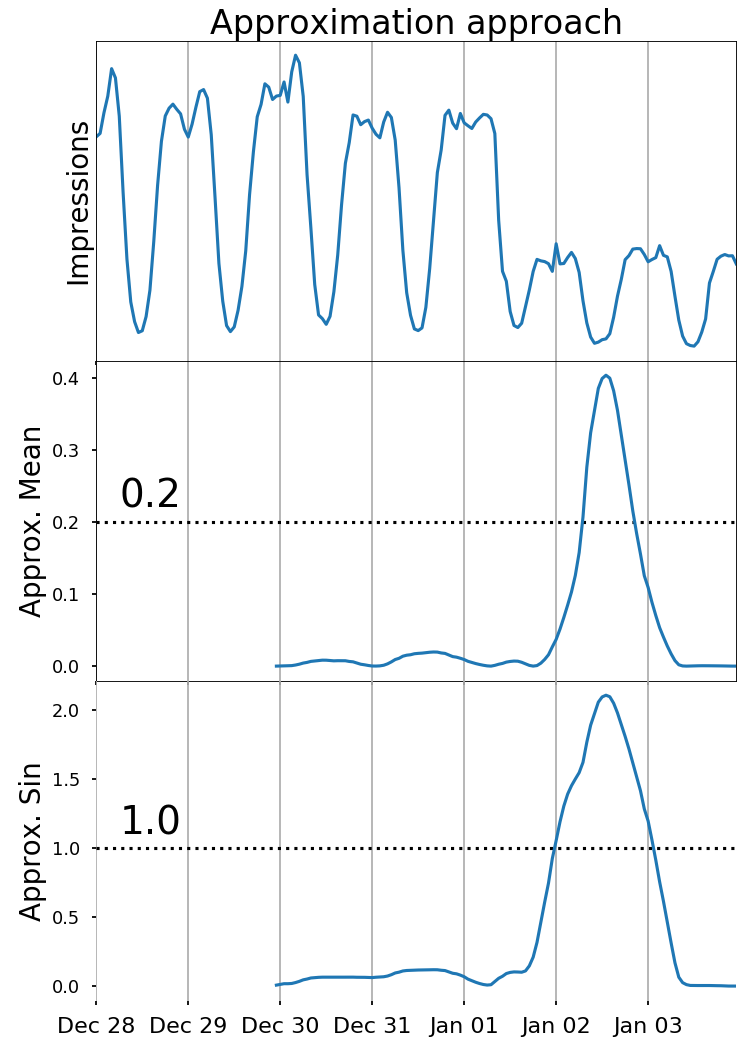
\includegraphics[height=6.5cm]{images/methods_comparison_1_2}
	\end{figure}
	
     \end{columns}

\end{frame}


\begin{frame}
    \frametitle{Applications to real data. Mean change}
  \begin{columns}[T,onlytextwidth]
      \column{0.5\textwidth}
\begin{figure}
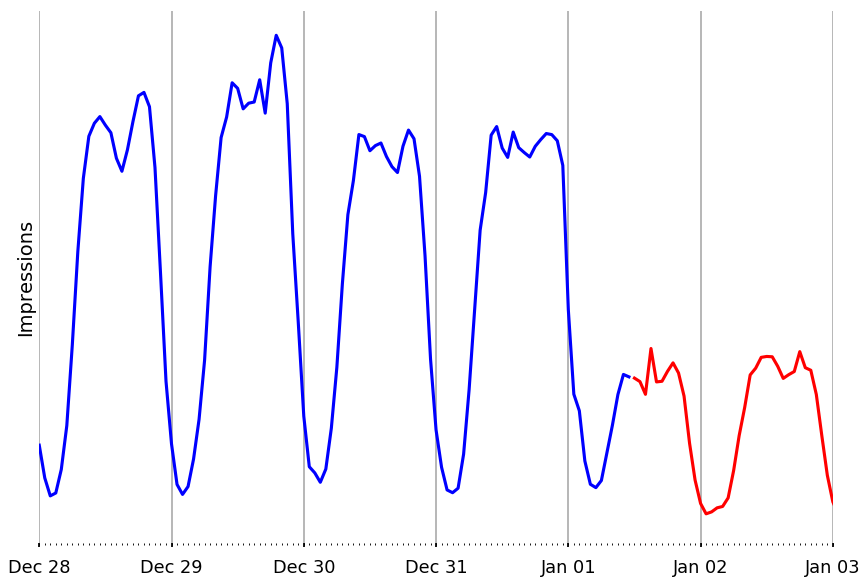
\includegraphics[scale=0.2]{images/methods_comparison_2}
\end{figure}
      \column{0.5\textwidth}
	    \begin{itemize}
	    	\item All models find significant change in mean pretty good
		\item Prediction approach with Mean model works worse here, because of relatively small window between no change and change point
	    \end{itemize}
     \end{columns}
\end{frame}



\begin{frame}
    \frametitle{Applications to real data. Outlier}
  \begin{columns}[T,onlytextwidth]
      \column{0.5\textwidth}
	\begin{figure}
	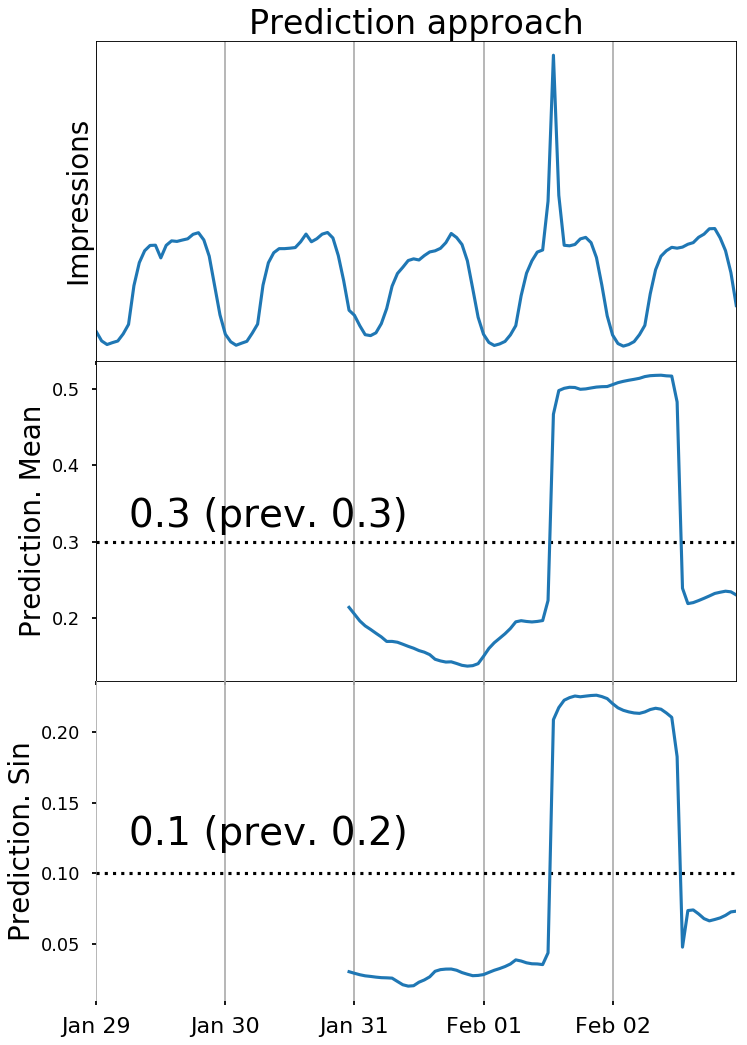
\includegraphics[height=6.5cm]{images/methods_comparison_2_1}
	\end{figure}
	
      \column{0.5\textwidth}
	\begin{figure}
	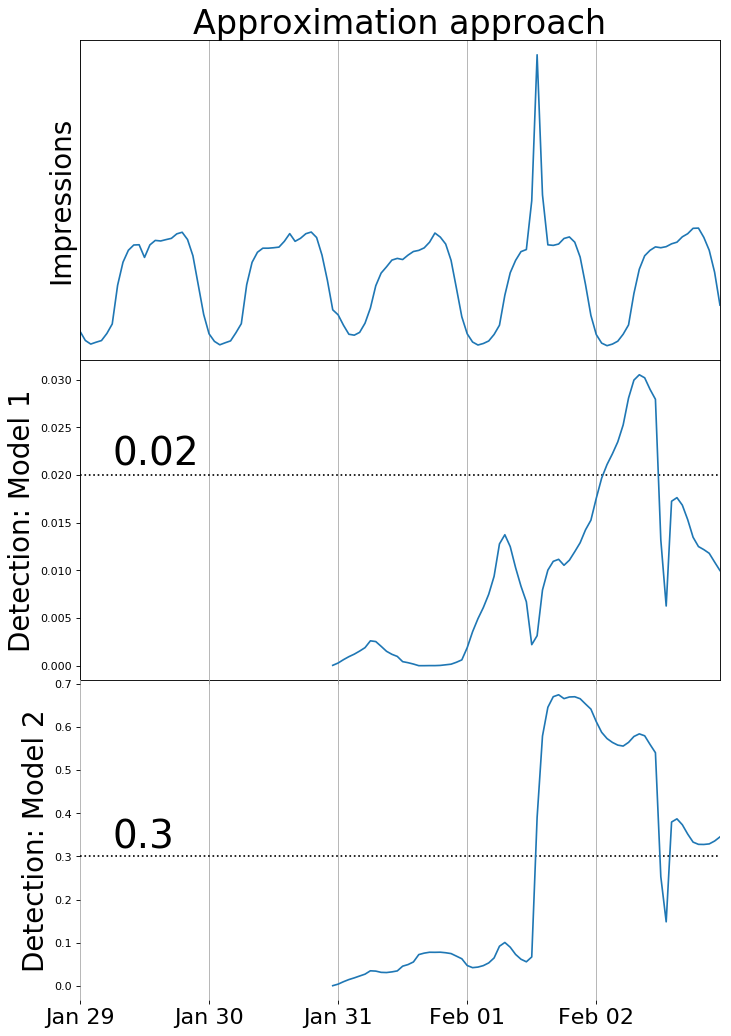
\includegraphics[height=6.5cm]{images/methods_comparison_2_2}
	\end{figure}
	
     \end{columns}

\end{frame}

\begin{frame}
    \frametitle{Applications to real data. Outlier}
  \begin{columns}[T,onlytextwidth]
      \column{0.5\textwidth}
	\begin{figure}
	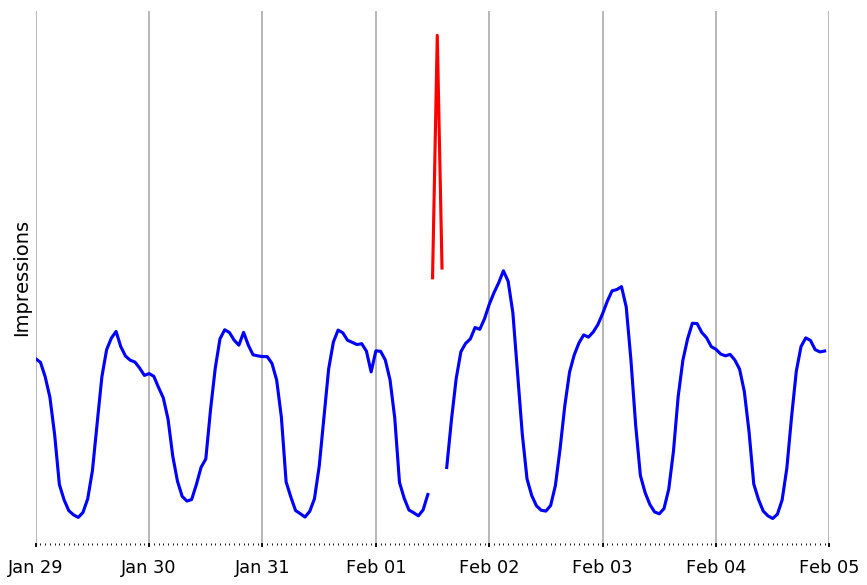
\includegraphics[scale=0.2]{images/methods_comparison_4}
	\end{figure}
      \column{0.5\textwidth}
	    \begin{itemize}
	    	\item Approximation approach with Mean model show noisy result
		\item Along with that, to detect such change with Approximation Mean we need to reduce threshold ten times
	    \end{itemize}
     \end{columns}
      
\end{frame}


\begin{frame}
    \frametitle{Applications to real data. Periodic component change}
  \begin{columns}[T,onlytextwidth]
      \column{0.5\textwidth}
	\begin{figure}
	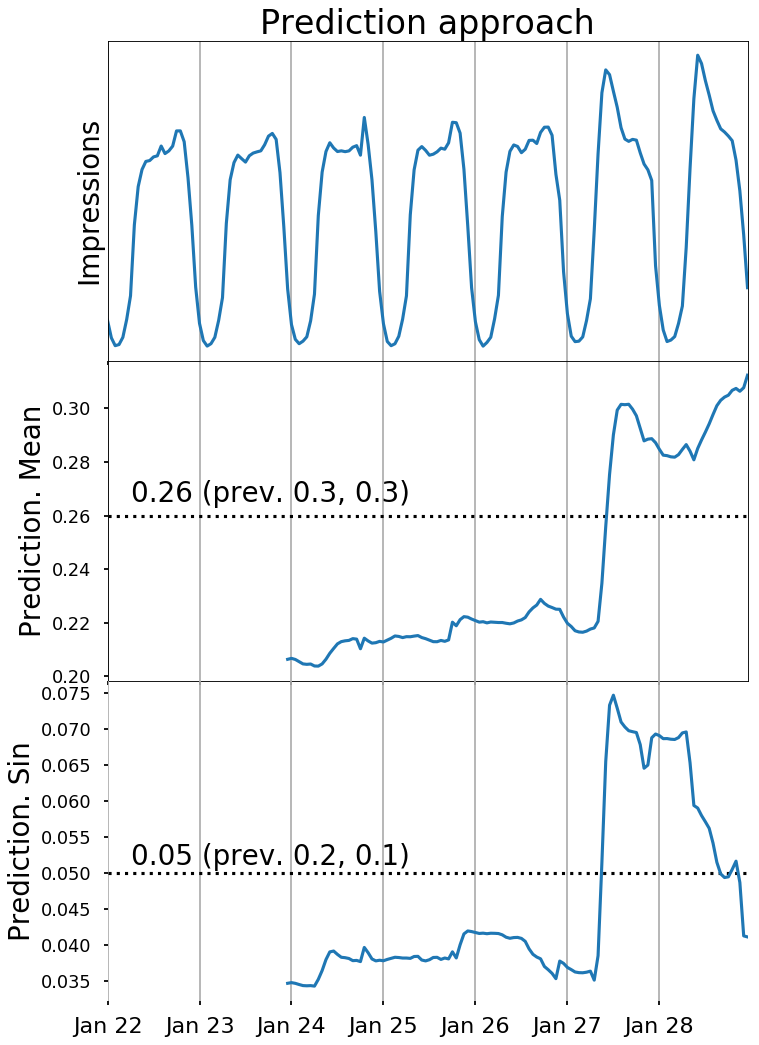
\includegraphics[height=6.5cm]{images/methods_comparison_3_1}
	\end{figure}
	
      \column{0.5\textwidth}
	\begin{figure}
	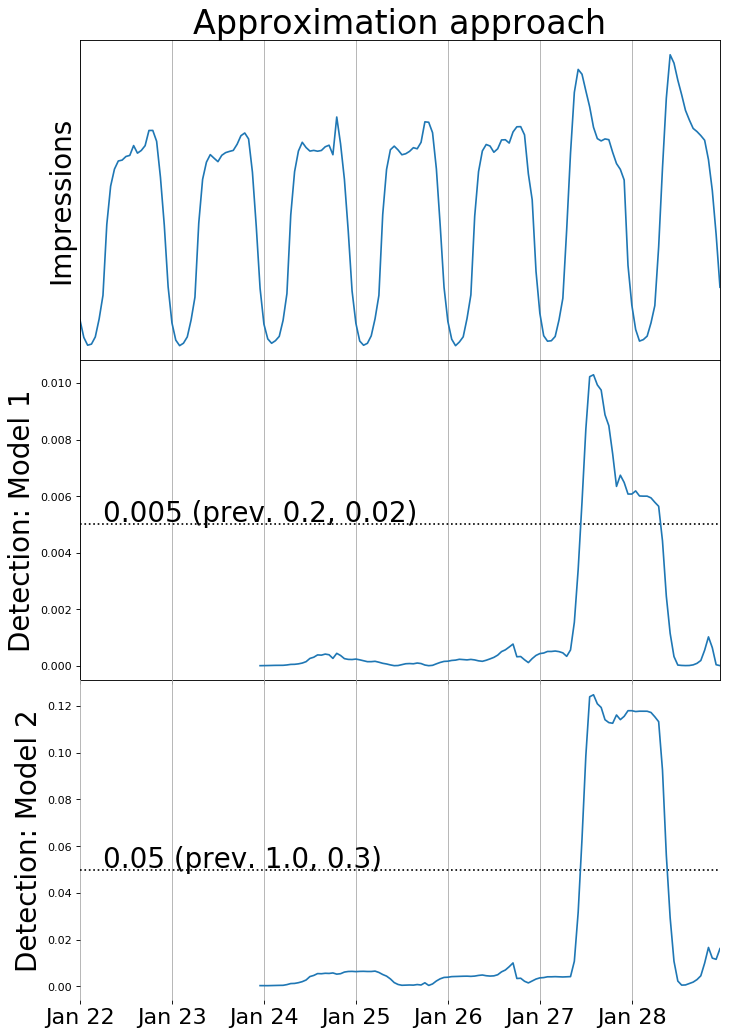
\includegraphics[height=6.5cm]{images/methods_comparison_3_2}
	\end{figure}
	
     \end{columns}

\end{frame}

\begin{frame}
    \frametitle{Applications to real data. Periodic component change}
  \begin{columns}[T,onlytextwidth]
      \column{0.5\textwidth}
	\begin{figure}
	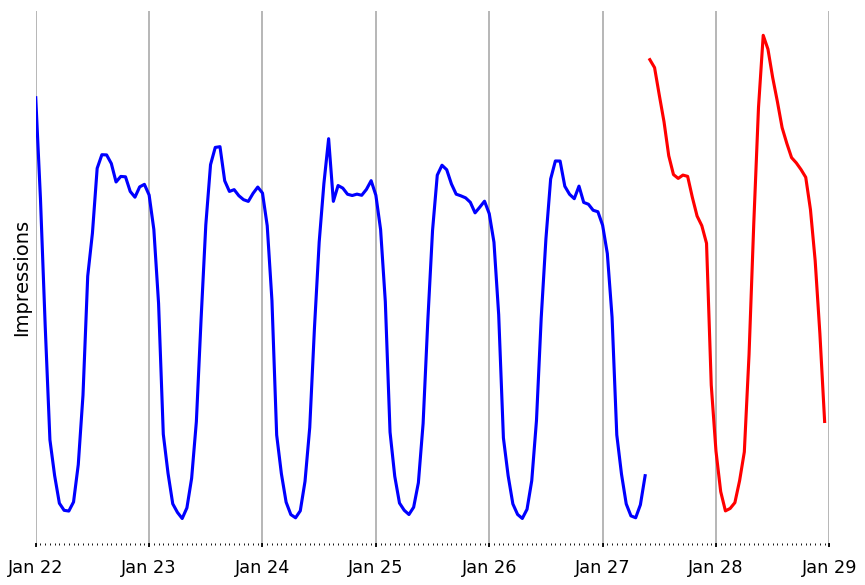
\includegraphics[scale=0.2]{images/methods_comparison_6}
	\end{figure}
      \column{0.5\textwidth}
	    \begin{itemize}
	    	\item To find detailed change point we need to reduce threshold significantly
		\item Cos model works better in such cases, because it is fitted to structure of time series
	    \end{itemize}
     \end{columns}
\end{frame}

\begin{frame}
    \frametitle{Applications to real data. Overview}

\begin{table}
\centering
Models thresholds
\begin{tabular}[t]{|p{8em}|p{5em}|p{5em}|p{5em}|p{5em}|}
\hline
  & Pred. Mean & Pred. Sin & Approx. Mean & Approx. Sin\\
\hline
Change in mean & 0.3 (0.25 - 0.35) & 0.2 (0.05 - 0.35) & 0.2 (0.01 - 0.4) & 1.0 (0.01 - 2.0)\\
\hline
Local change (outlier) & 0.3 (0.2 - 0.5) & 0.1 (0.05 - 0.2) & 0.02 (0.01 - 0.03) & 0.3 (0.01 - 0.6)\\
\hline
Change in periodic component & 0.26 (0.22 - 0.30) & 0.05 (0.04 - 0.07) & 0.005 (0.001 - 0.010) & 0.05 (0.01 - 0.12)\\
\hline
\end{tabular}
\end{table}

\begin{itemize}
	\item Prediction approach looks less robust than approximation, because it has less distance between lowest and highest scores.
	\item Mean model finds change points well. But when we need to find some changes, which does not affect mean of time series, we need to apply some other models
	\item You should choose threshold depending on how detailed changes would you like to find
\end{itemize}

\end{frame}

\begin{frame}
    \frametitle{Search method}
We can search for change points differently
\begin{itemize}
	\item Force (always from left to right). Good for alerts.
	\item Back (always from right to left). Good for forecast.
	\item Force and back (time series and each time series searched from both ends). Good for analysis of historical data.
\end{itemize}

  \begin{columns}[T,onlytextwidth]
      \column{0.5\textwidth}
      Force method:
	\begin{figure}
	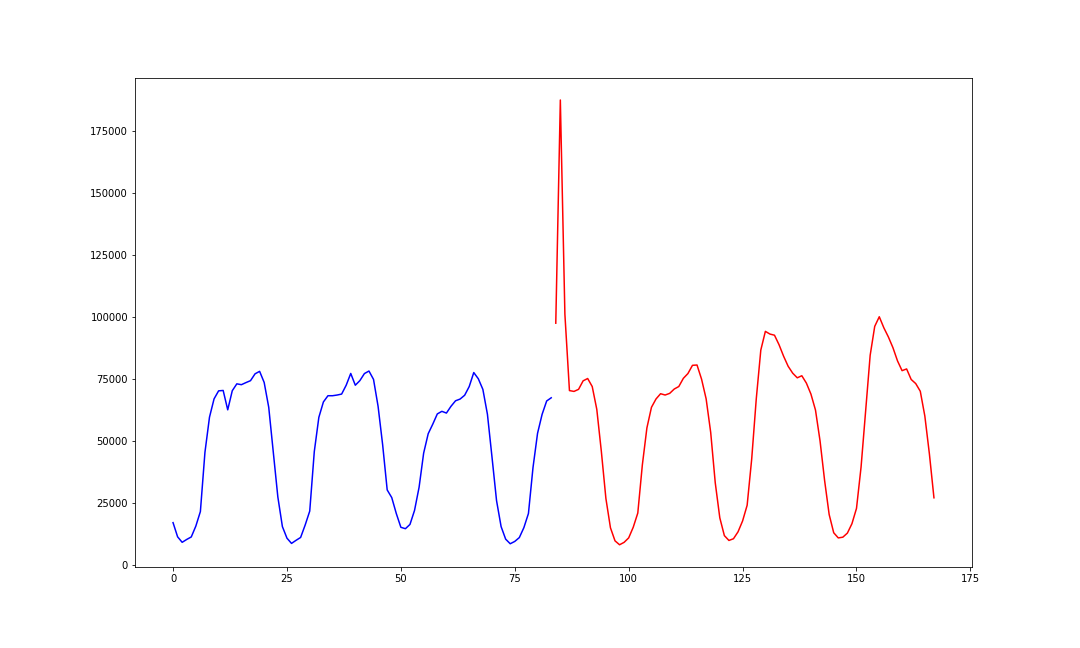
\includegraphics[scale=0.15]{images/022_point_cp_detected}
	\end{figure}
      \column{0.5\textwidth}
      Force and back method:
	\begin{figure}
	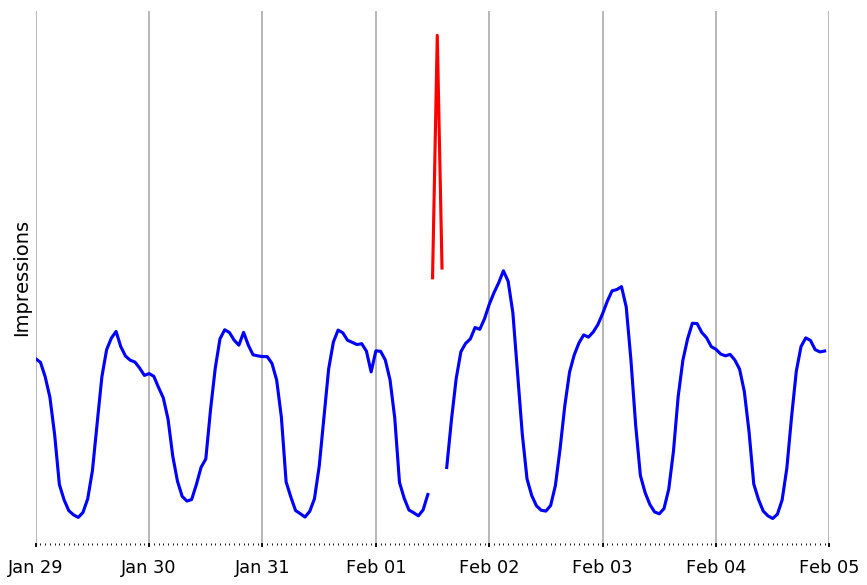
\includegraphics[scale=0.15]{images/methods_comparison_4}
	\end{figure}

     \end{columns}


\end{frame}

\begin{frame}
    \frametitle{Applications to real data. Long time series}
For the final model we chose Approximation approach with Mean model, threshold = 0.4 and force-back search method.
Let's take a look how does it work on a real long time series:
  \begin{columns}[T,onlytextwidth]
      \column{0.5\textwidth}
	\begin{figure}
	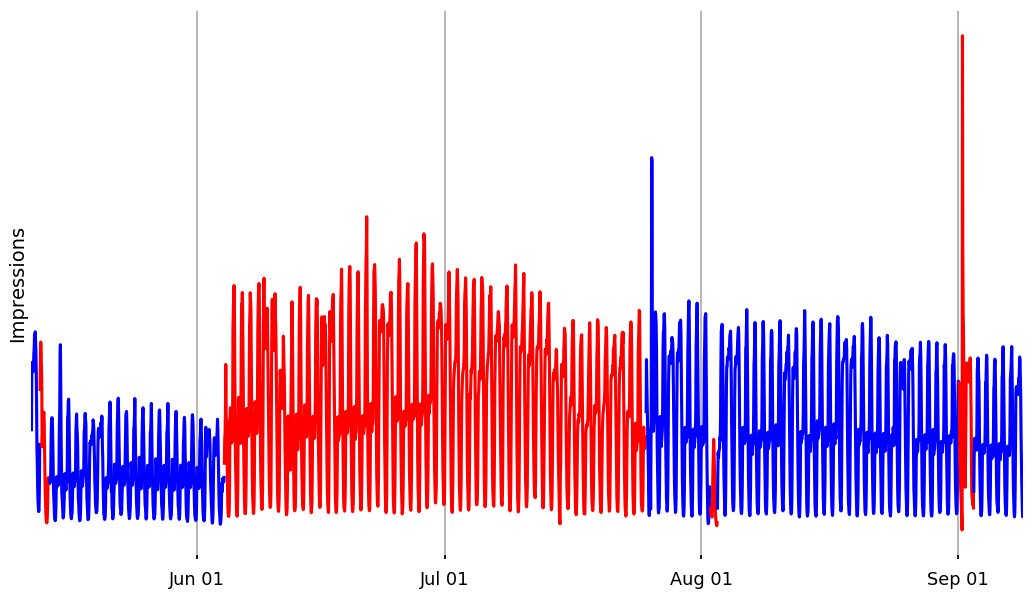
\includegraphics[scale=0.16]{images/long_ts_1}
	\end{figure}
      \column{0.5\textwidth}
      	\begin{figure}
	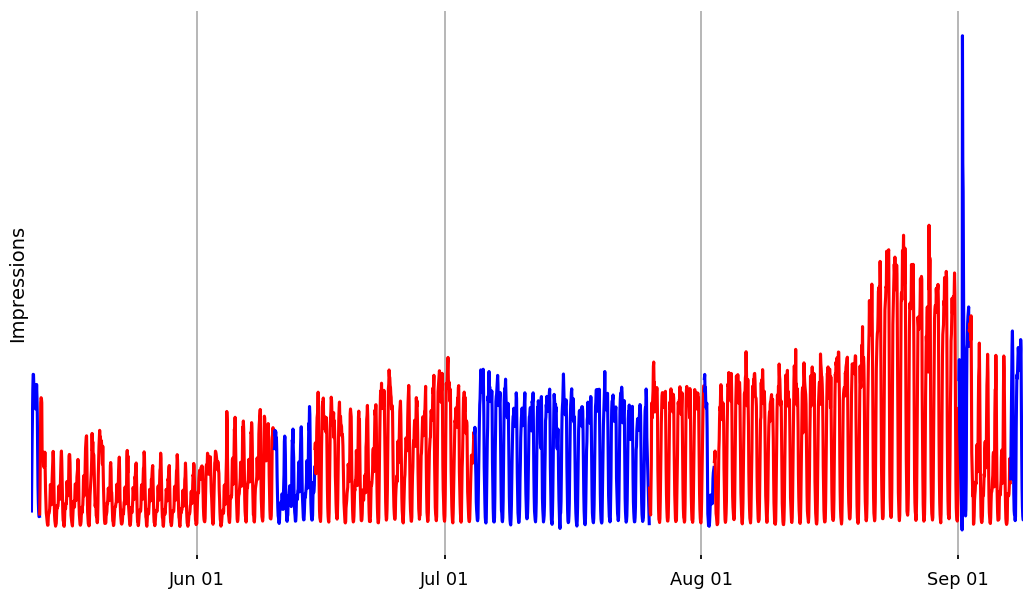
\includegraphics[scale=0.16]{images/long_ts_2}
	\end{figure}

     \end{columns}
\end{frame}


% \begin{frame}
%    \frametitle{What about trend change?}

% Above models don't really work here:

%   \begin{columns}[T,onlytextwidth]
%       \column{0.5\textwidth}
% 	\begin{figure}
% 	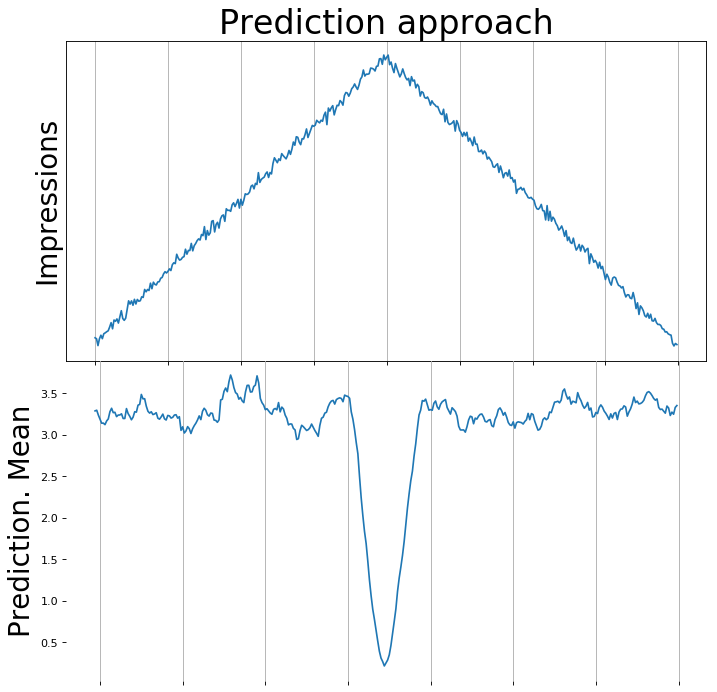
\includegraphics[height=5.5cm]{images/methods_comparison_4_1}
% 	\end{figure}
	
%       \column{0.5\textwidth}
% 	\begin{figure}
% 	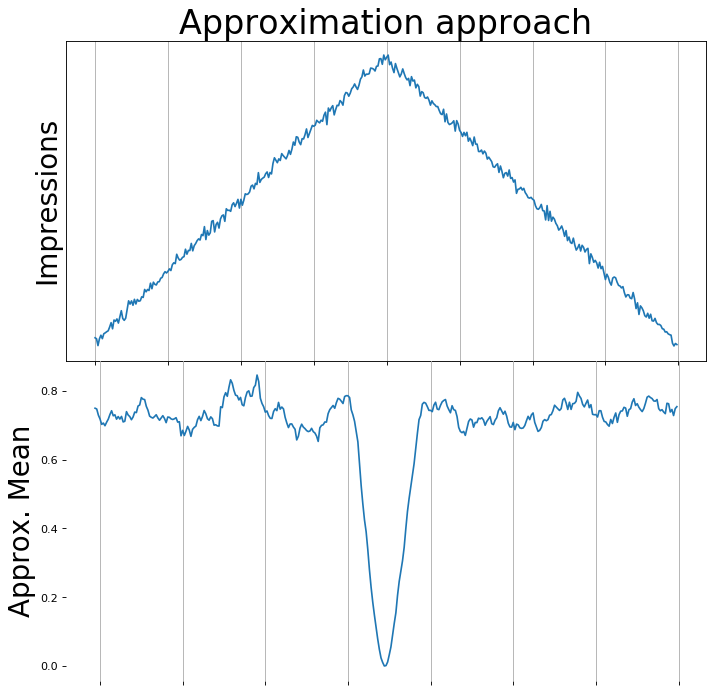
\includegraphics[height=5.5cm]{images/methods_comparison_4_2}
% 	\end{figure}
	
%      \end{columns}

% \end{frame}

% \begin{frame}
%     \frametitle{Model for trend change detection}
    

% We can just add linear trend part (B) to our model:
% $$ \mathrm{X} = a + Bn + C\cos(2\pi \frac{n}{24}) + S \sin(2\pi \frac{n}{24}) + \epsilon $$

% \begin{figure}
% 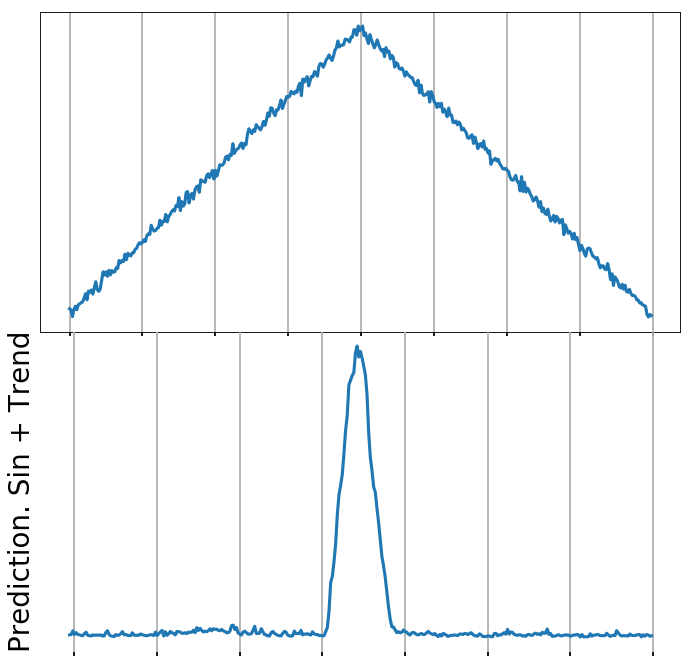
\includegraphics[scale=0.25]{images/methods_comparison_5_1}
% \end{figure}

% To allocate trend change we can aggregate data on daily level. Then apply change point detection with linear regression (as an example) model
% \end{frame}


\begin{frame}
    \frametitle{How to choose best parameters?}


Supervised machine learning techniques can be applied if the data are tagged by change-points.
\newline

We can estimate parameters mentioned above compare quality of change point detection using cross validation.
\newline
Quality can be estimated as sum of distance between real indexes and estimated indexes normalized by length of time series: $$\sum_{i=1}^K \frac{|\widehat{t_i} - t_i|}{N}$$	

It works perfectly, when our time series is tagged with change points.

 \end{frame}

\begin{frame}
    \frametitle{Machine learning for parameters estimation}

In real world there is no objectively good or bad tagging in this problem. So sometimes it is hard to tag the time series.

\begin{figure}
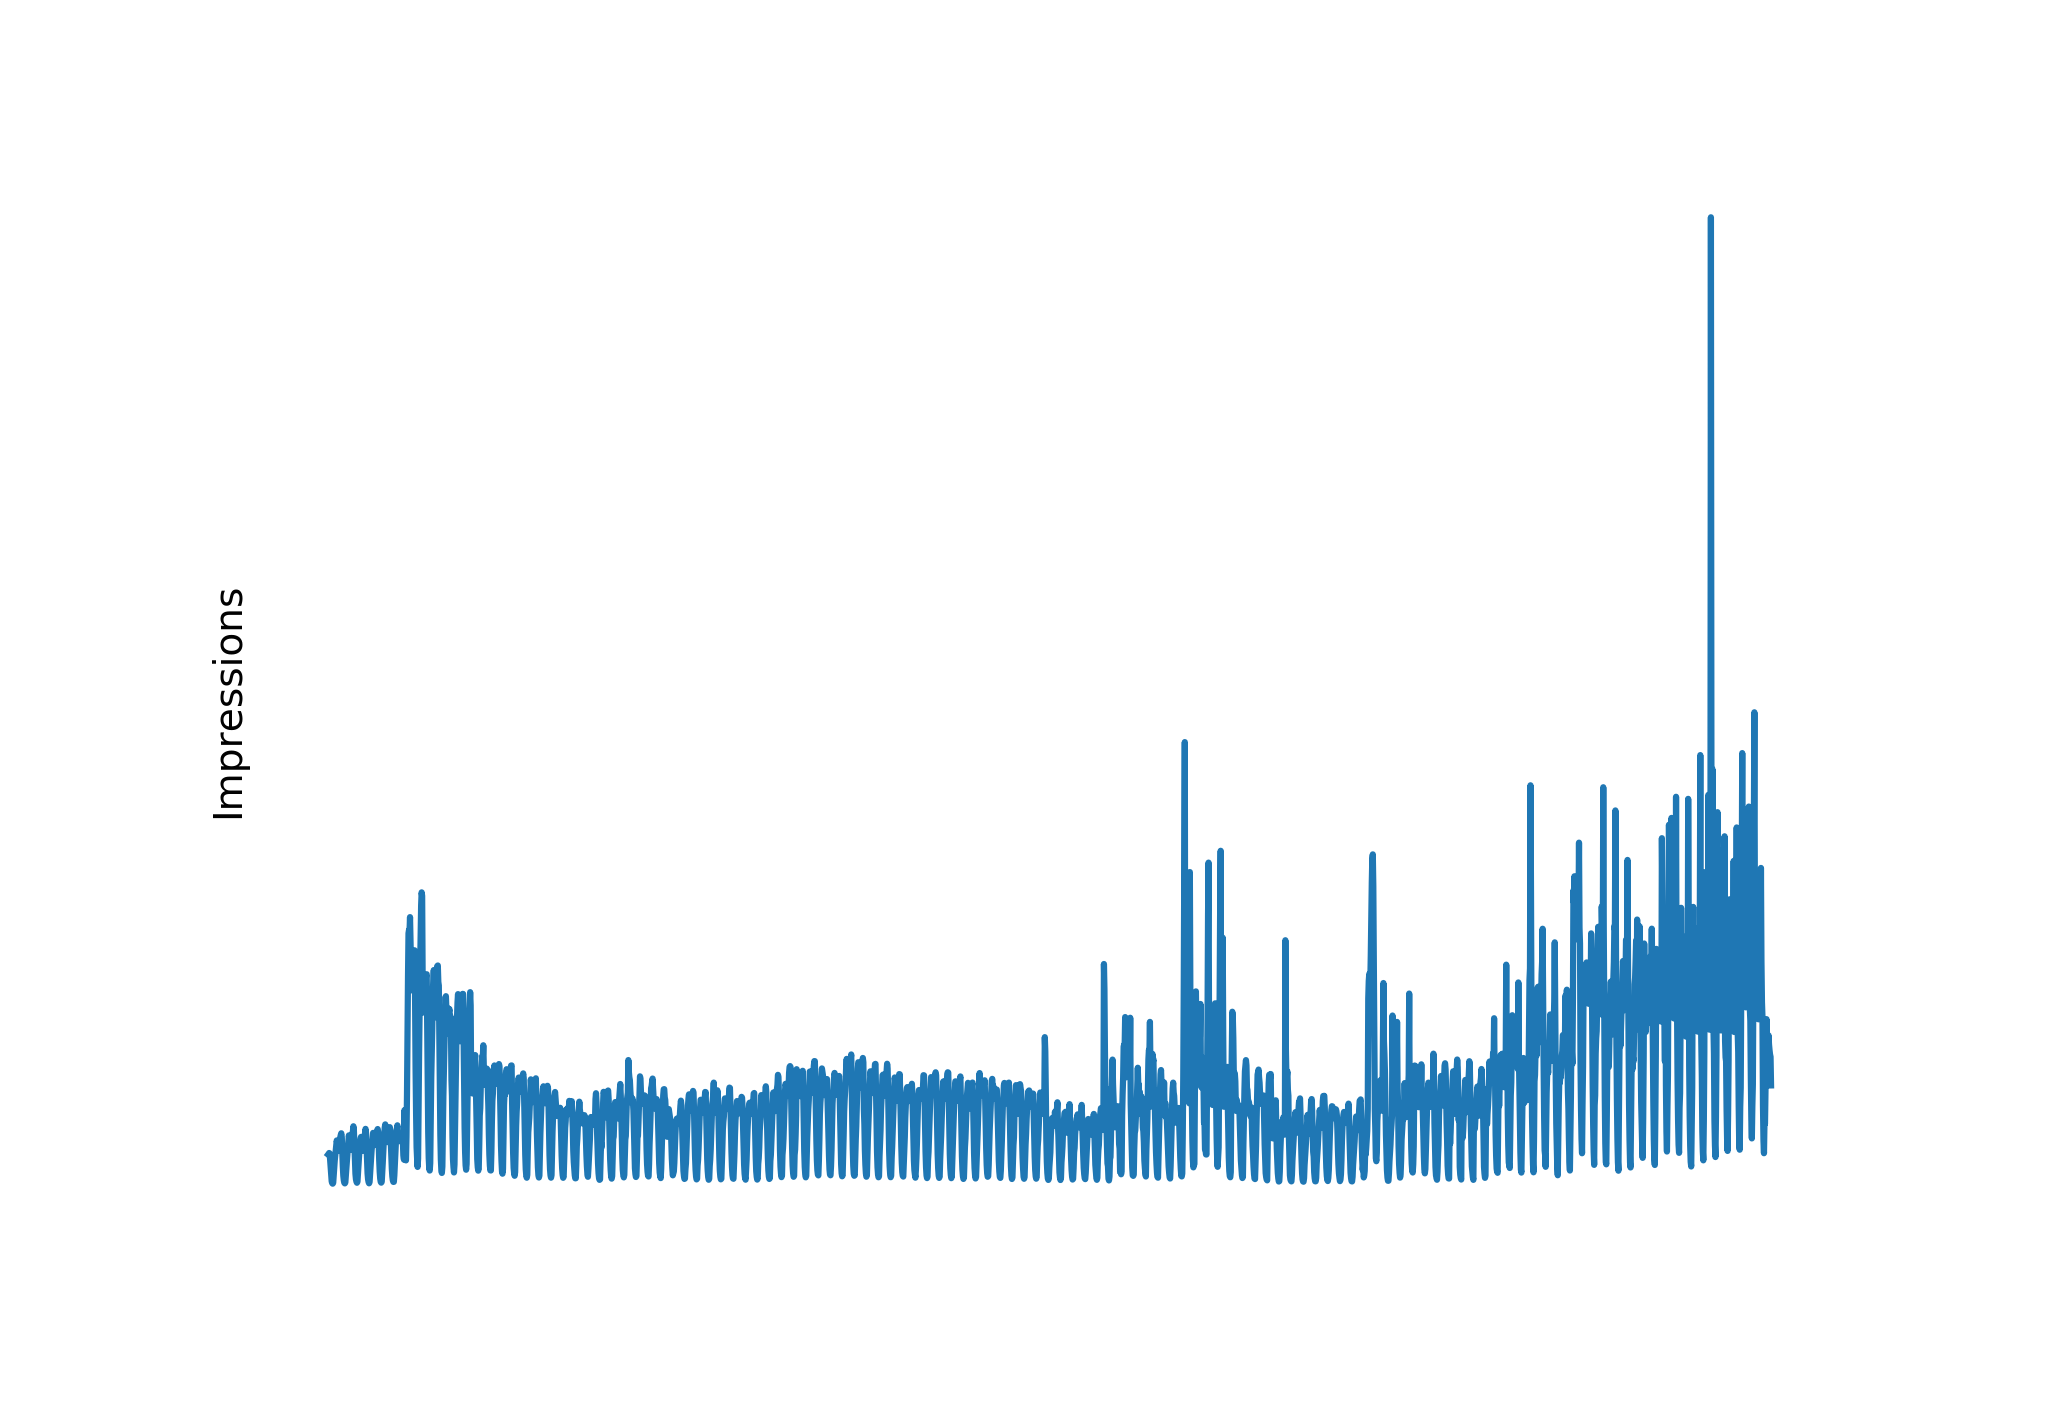
\includegraphics[scale=0.2]{images/examples_tagging}
\end{figure}

The possible solutions:
	    \begin{itemize}
	    	\item Tag it accordingly to what's important for business
		\item Estimate quality on higher level of task
	    \end{itemize}

 \end{frame}



\begin{frame}
    \frametitle{Airpush experience}
    
All these methods allow us to construct alert system which consists of two parts:

 \begin{itemize}
	    	\item Hourly level model, which allocates changes in mean, variance, periodic component and detects anomalies
		\item Daily level model which allocates changes in trend
\end{itemize}

We can split overall impressions time series by any important dimension, such as countries, ad formats, applications, etc.
Applying described methods can help us to identify change points automatically in every big enough country/applications/application/ad format time series.
\newline
In addition, we can adjust thresholds adaptively by monitoring for false alerts.

\end{frame}

\begin{frame}
    \frametitle{Next steps}
    
But we can move forward. Instead of plain alerts we can develop smart alerts system.
Instead of sending notification on each separate case (which could be a lot of at once). It aggregates alerts and send you only a summary, such as:

 \begin{itemize}
	    	\item Countries: 167 out of 196 had change
		\item Ad formats: 6 out of 8 had change
		\item Applications: 1 out of 3000 had change
\end{itemize}

It means that something affected almost all countries and almost all ad formats, \textbf{but} only one application. That is why most probably real root of change is the application, so we want to be notified only about this application.

\end{frame}


\begin{frame}
    \frametitle{Conclusion}

	    \begin{itemize}
	    	\item Change point detection system can help us to react on significant change fast
		\item There are many parameters and methods, but any parameter can be tuned iteratively
		\item Scope of application much wider than alert system
	    \end{itemize}

 \end{frame}


% \begin{frame}
%     \frametitle{Conclusion}

% 	    \begin{itemize}
% 	    	\item Main approaches works well on the real data and are good for different applications
% 		\item Wisely choosing of applicable model is important
% 		\item We can choose threshold which applicable to our task
% 		\item Aggregation of periods can help to find more general changes
% 		\item Change point detection system can help us to react on significant change fast
% 		\item Accurate tagging will allow to estimate detection quality
% 	    \end{itemize}

%  \end{frame}


\end{document}
